

\chapter{LazyGraph 性能提升规律研究}
在前面的章节中我们提到延迟数据一致性方法遗留的主要问题是如何找到合适的开启策略从而得到相对最优的性能提升。
为此,本章对不同开启策略下得到不同程度的性能提升这一问题进行了研究,并通过实验得到了结论:
性能提升主要受冗余计算影响,不同开启策略下存在不同程度的冗余计算,从而得到了不同程度的性能提升。
通过这一结论,本文对延迟数据一致性方法的性能提升的规律有了更深刻的认识。

本章将首先通过具体的例子对比急切数据一致性方法和延迟数据一致性方法来展示后者性能收益的来源,
然后再具体分析这个例子来说明延迟数据一致性方法中存在的冗余计算这一现象。
最后通过具体的实验数据论证正是冗余计算造成了不同开启策略下延迟数据一致性方法会得到不同程度的性能提升。



\section{冗余计算对 LazyGraph 的性能收益的影响}
\subsection{延迟数据一致性方法带来性能收益}
% \section{算法视角下的延迟数据一致性方法的性能收益来源}
% 为了解决LazyAsync的优化问题,本文首先对延迟数据一致性这种方法性能收益的来源进行了研究。
关于延迟数据一致性方法如何拿到性能收益,我们之前的工作其实已经有所解释。
之前的解释从分布式计算系统的角度阐述,把性能收益归因于迭代轮次和通信量的减少。
但是这种解释不足以说明这种方法为何有时性能收益较高有时却较低,以及为何有时迭代次数减少计算时间却并没有明显减少。


本文继续从具体算法用例的角度来解释,延迟数据一致性方法具体是减少了哪些部分的全局同步。
为此,本文以 单源最短路径算法(Single Source Shortest Path,SSSP)算法为例,在一个小图上分别以 eager data coherency 和 lazy data coherency 的方式运行算法。
这样的对比直观地揭示出了从具体的算法角度而言,LazyAsync 方法究竟是减少了哪些部分的全局同步。
同时,这里的对比过程也为后边的冗余计算问题的提出打下了基础。


为此,我们需要先对图计算中的 SSSP 算法进行介绍。
为了支持各种图算法,大规模图计算框架往往需要在底层图计算系统和上层具体的图算法之间进行抽象。
PowerGraph从单个顶点的角度出发\cite{McCune@CS15},把所有的图算法抽象为Gather,Apply,Scatter三个阶段。
用户使用框架提供的GAS编程接口可以实现各种图算法。
算法\ref{alg:SSSP}中描述了基于GAS编程接口实现的SSSP算法。
Gather阶段,提供了顶点访问周边邻居并拉取信息的接口,SSSP中不需要这个过程。
Apply阶段,提供了根据收到的消息及拉取到的信息,修改顶点上的数据的接口,SSSP中每个顶点根据收到的信息更新自己到 source 的距离。
Scatter阶段,提供了顶点访问周边邻居并推送信息的接口,SSSP中,每个顶点根据自己更新的距离,判断是否进一步激活自己的邻居顶点。


\begin{algorithm}[!htbp]
  \small
  \caption{基于GAS接口实现的 SSSP 算法\cite{low2013graphlab}}\label{alg:SSSP}
  \begin{algorithmic}[1]
    \Procedure{SSSP}{G(V,E,D)}
    \State $gather(D_u,D_{(v,u)},D_v): return$     \Comment{gather\_nbrs: empty}
    \State $sum(a,b) : return a\bigoplus b $ \Comment{(min(a,b))}
    \State $apply(D_u, new\_dist): 
      \qquad D_u = new\_dist$
    \State $scatter(D_u, D_{(u,v)}, D_v):$     \Comment{scatter\_nbrs: all\_out\_nbrs}
    \If{ $ changed(D\_v) $ }
      \State { $ active(v, D_u+D_{(u,v)})$ }
    \EndIf
    \EndProcedure
  \end{algorithmic}
\end{algorithm}


\subsubsection{eager data coherence 中的SSSP算法}
下面以一个小图来具体说明 SSSP 在图计算框架中采用 eager data coherence 方式实现的同步引擎上的执行过程。
图\ref{fig:sssp-sync-iter}中展示了在一个小的输入图上,SSSP算法的执行过程。
这个小图由14个顶点和19条边构成,划分在3台机器上,以0号顶点为source,计算其他顶点到source的最短距离。
系统一开始会把消息值0发送给0号顶点,进而激活0号顶点,把0号顶点作为活跃点参与计算。

在第0轮迭代的apply阶段,0号顶点会根据收到的消息把自己顶点上的数据更新为0,
在第0轮迭代的scatter阶段,0号顶点的master部分和mirror部分会激活自己的本地邻居。
反映在图中就是,机器0上的master 0 激活了自己的本地邻居 master 1 和 mirror 11,
机器2上的mirror 0 激活了自己的本地邻居mirror 41 和 mirror 31。
这样,第0轮迭代后,0号顶点的1,11,31,41这4个邻居都被激活并发送了消息值1
(这里需要说明的是边上值缺省为1,所以发送了值1)。
消息发送完毕后第0轮迭代完成,系统进入第1轮迭代。

在进入第1轮的GAS实际计算之前,图计算的底层引擎会对系统中存在的消息进行收发处理,
把每一条消息送到其接收者master部分所在的机器上,并把接收者标记为新一轮的活跃点。
在消息处理完毕后,底层引擎会统计活跃点的数量,如果为0,那么迭代结束,运算完成,
如果不为0,那么继续进行GAS运算。
反映在图中,第1轮迭代,顶点1,11,31,41成为活跃点。
在第1轮迭代的apply阶段,机器0上的master 41,master 1根据收到的消息把自己顶点上的数据更新为1,
机器1上的master 11根据收到的消息把自己顶点上的数据更新为1,
机器2上的master 31根据收到的消息把自己顶点上的数据更新为1。
Apply阶段结束后,系统采用急切一致性的方法,把1,11,31,41号顶点master部分的信息立即同步到其他mirror顶点上去,
这样顶点的master部分和mirror部分就立即实现了一致性。
在scater阶段,1,11,31,41这4个活跃点的master部分和mirror部分都会执行scatter操作去激活自己的本地邻居。
反映到图中,
机器0上的mirror11会激活它的邻居master2,master 1则由于本地没有邻居不进一步激活,
机器1上的master 11也由于本地没有邻居不进一步激活,
机器2上的mirror 41则会激活本地邻居master 61,mirror 1则会激活本地邻居mirror 2。

这样这些被激活的2号顶点和61号顶点则会进一步作为第2轮的活跃点进行计算,直到最后系统中没有活跃点,运行结束。
最终在经过10轮迭代之后,图中的顶点都求得了到source的最短路,运算结束。


\begin{center}
  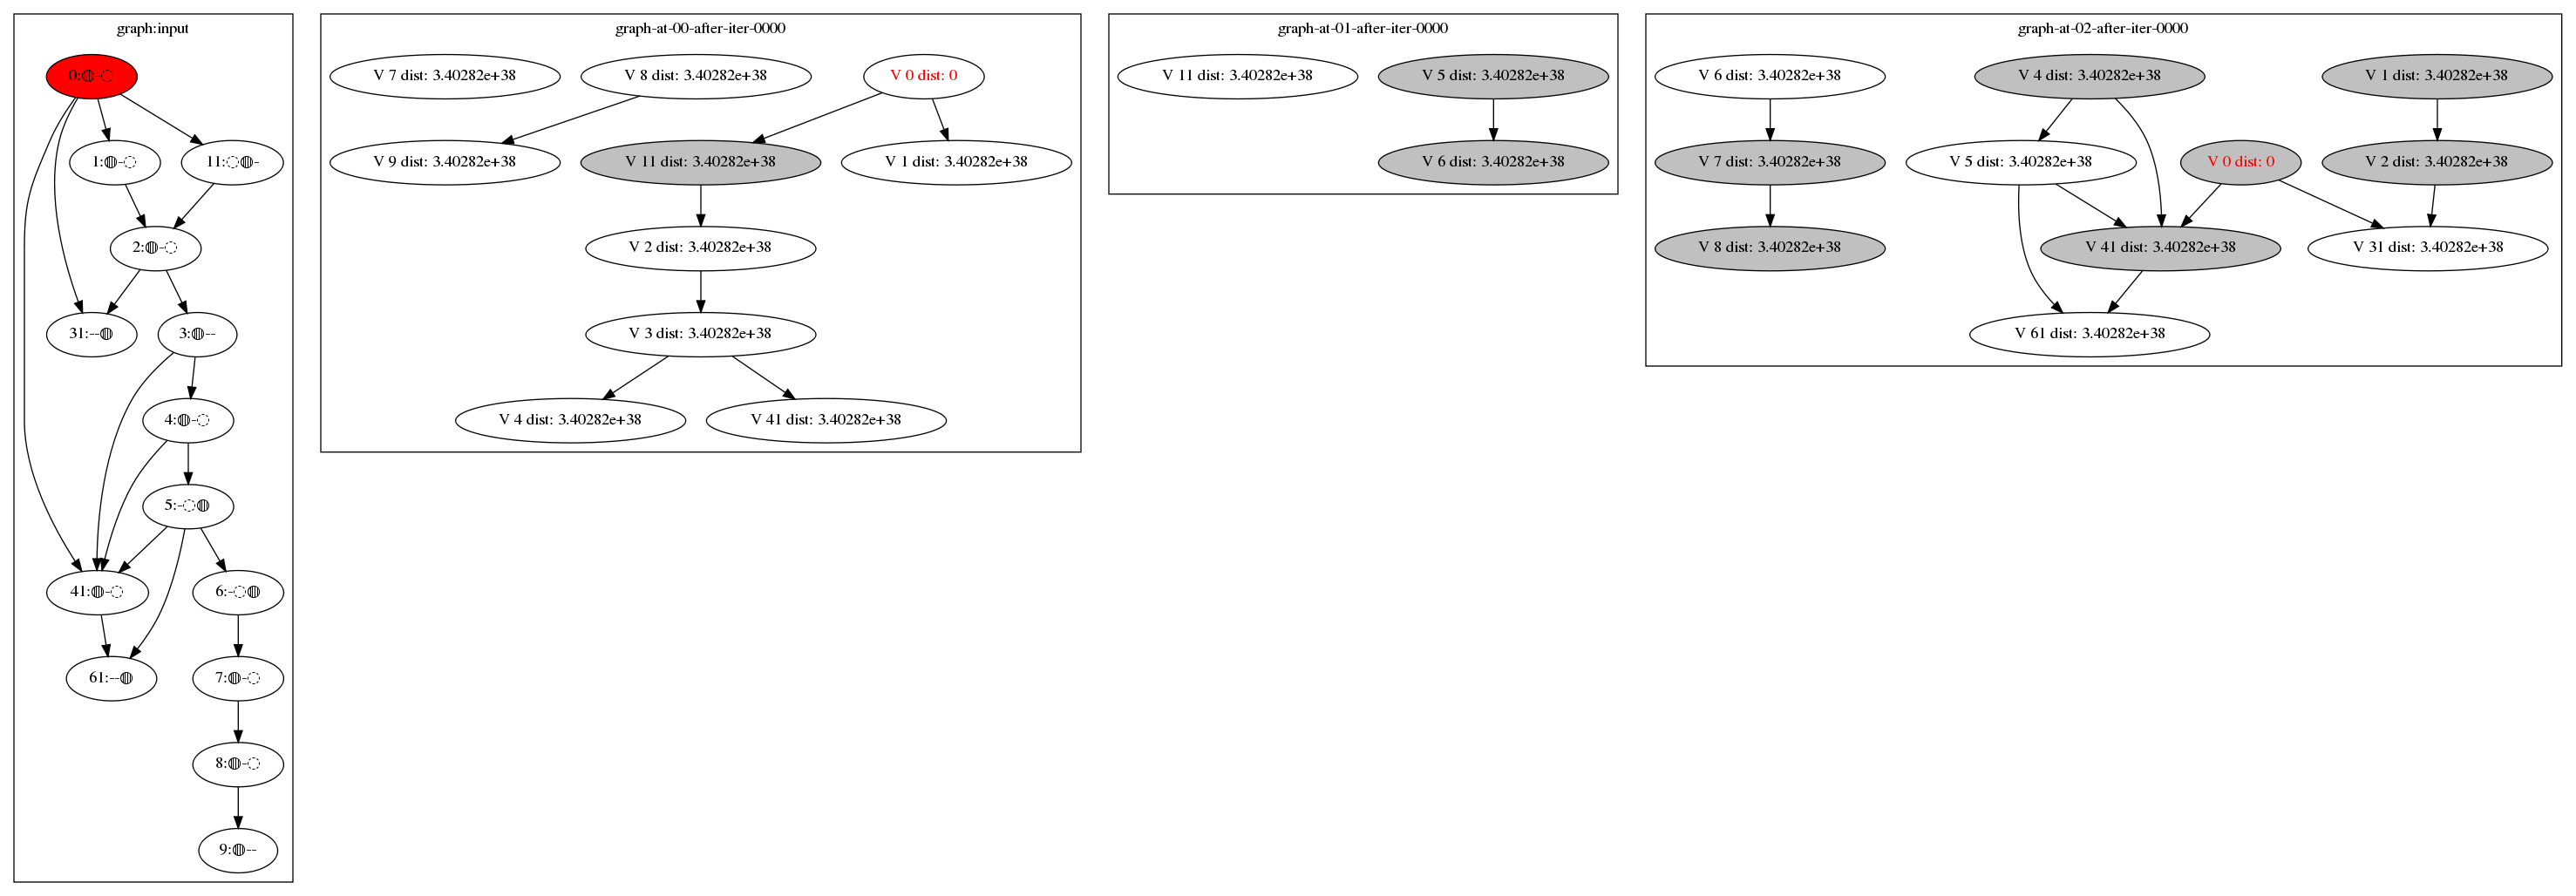
\includegraphics[width=0.8\textwidth]{sync-iter0.png}
  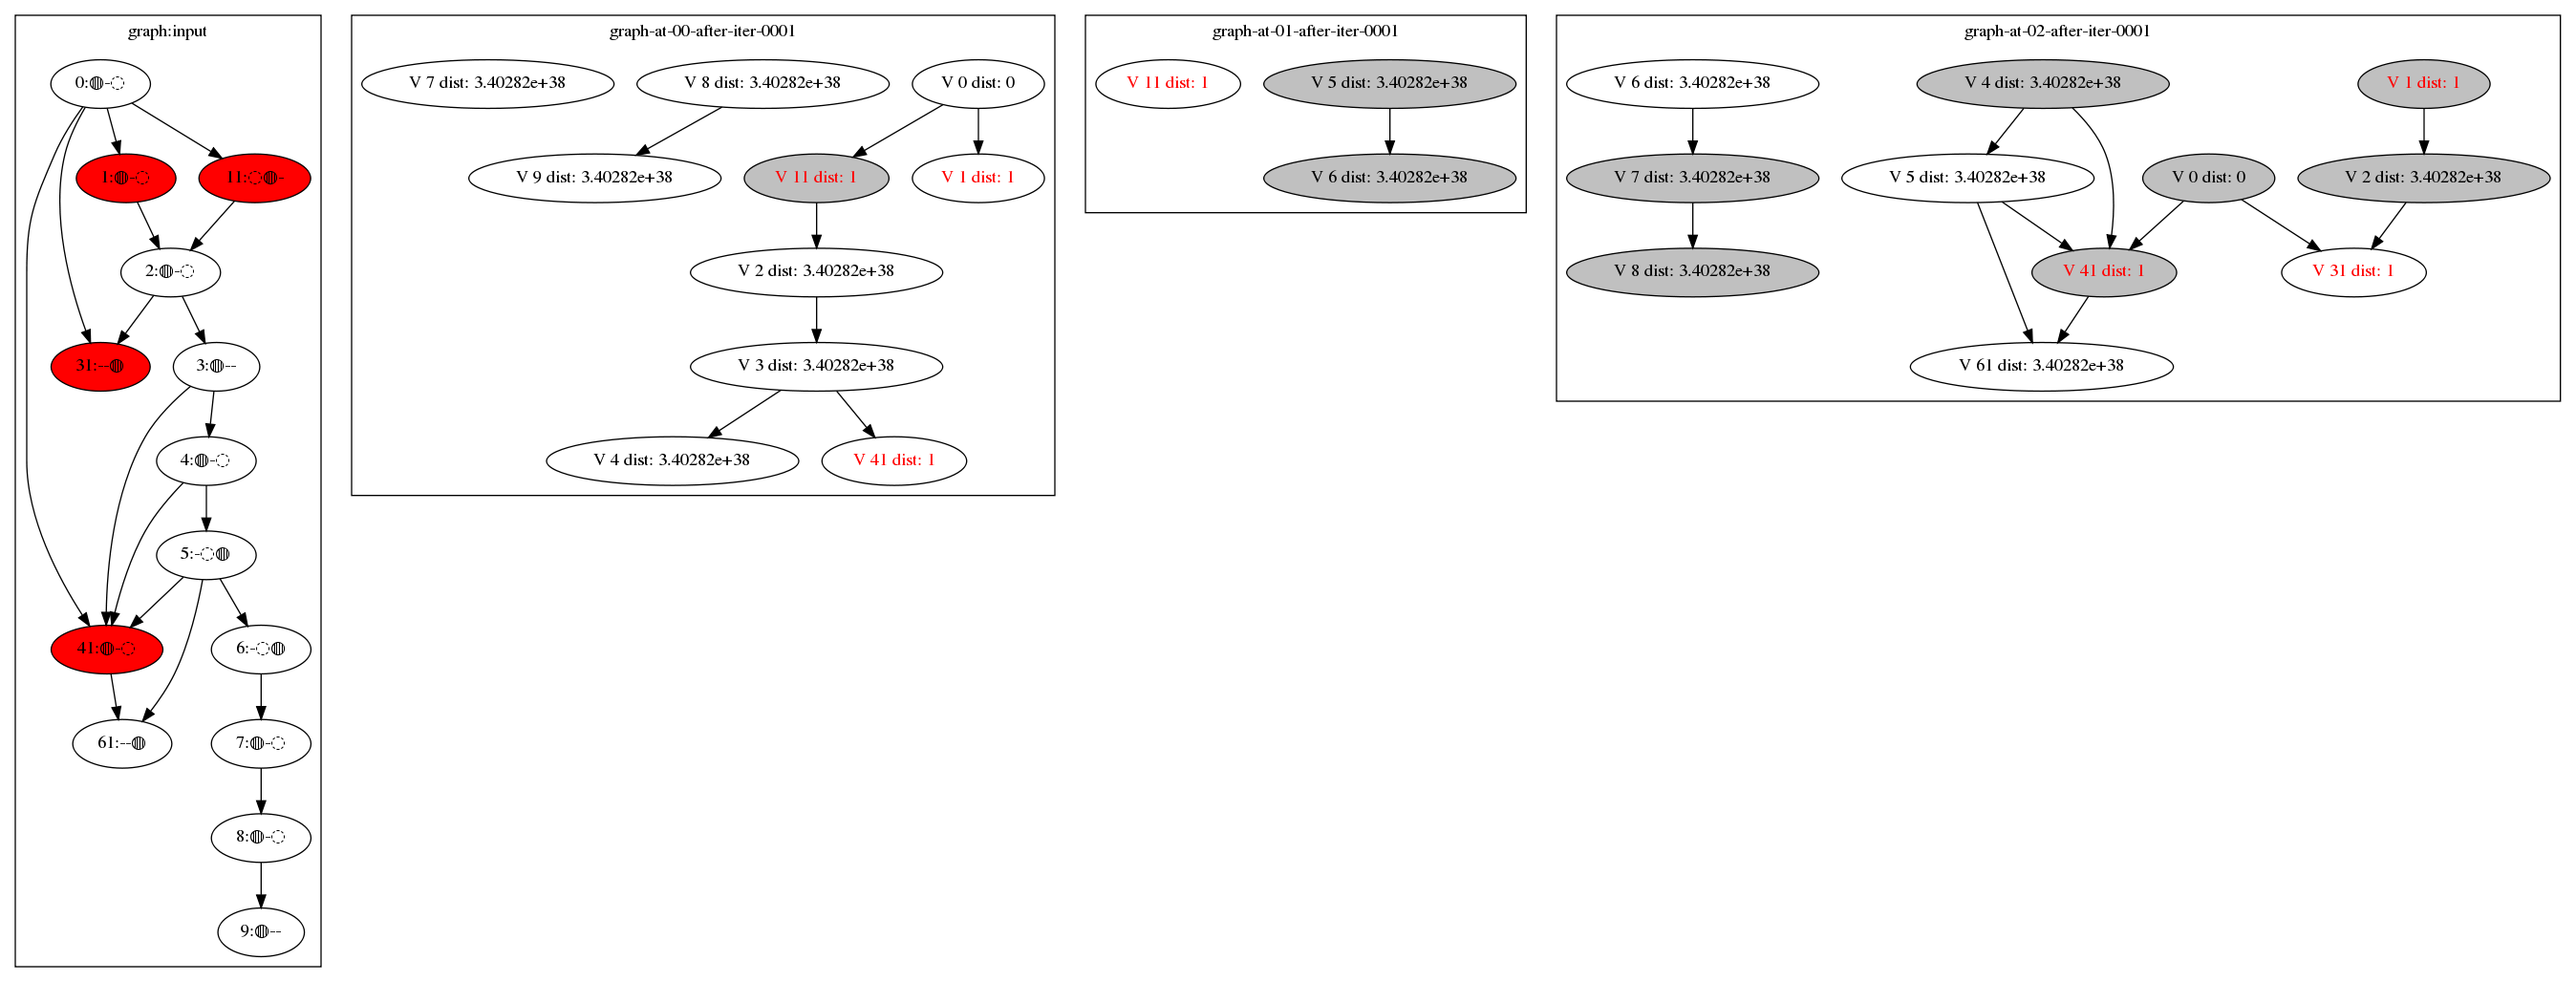
\includegraphics[width=0.8\textwidth]{sync-iter1.png}
  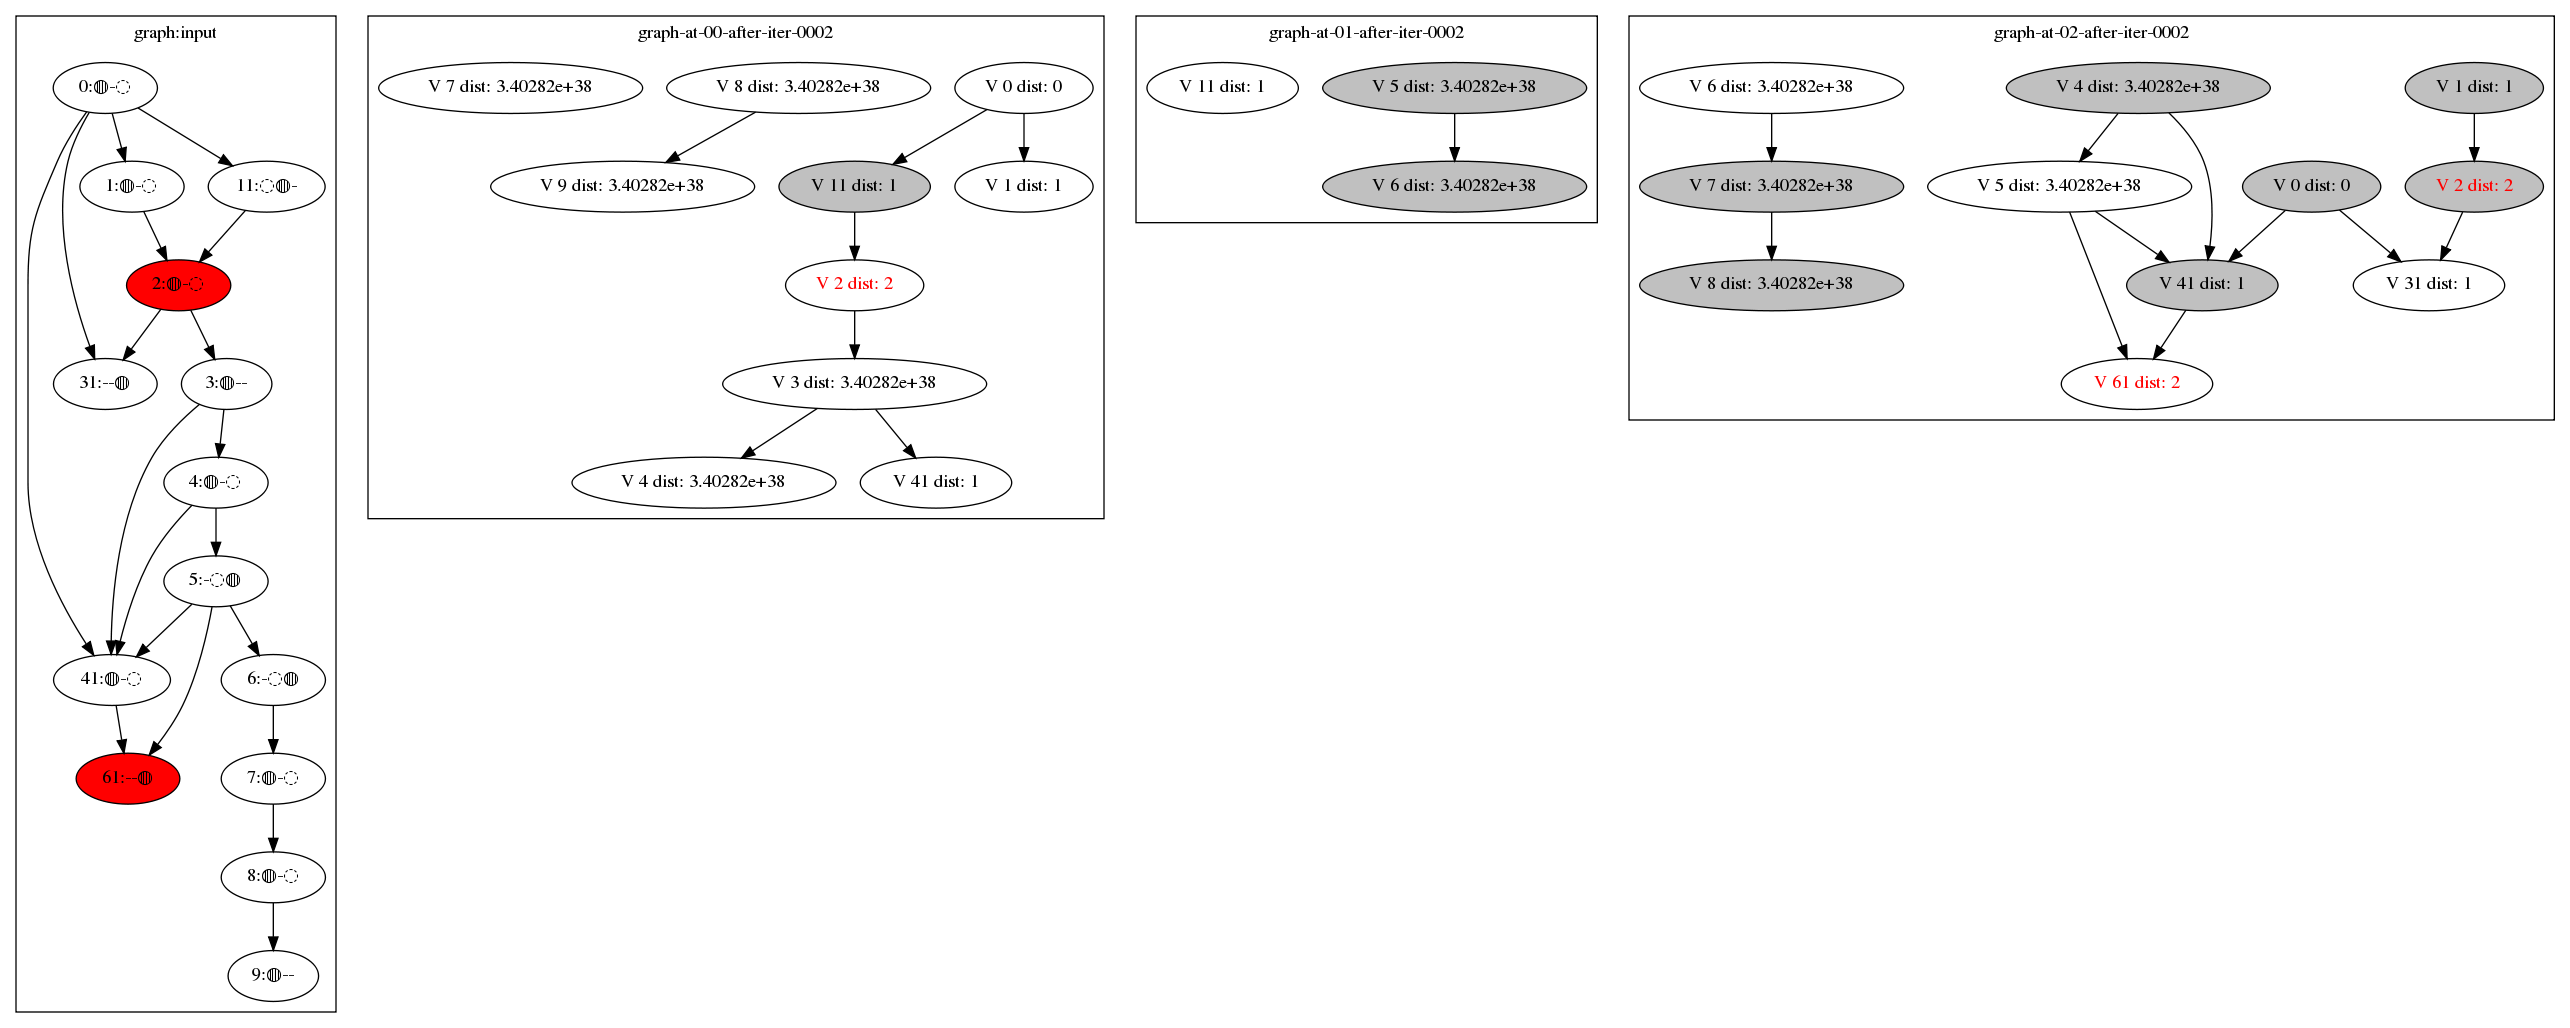
\includegraphics[width=0.8\textwidth]{sync-iter2.png}    
  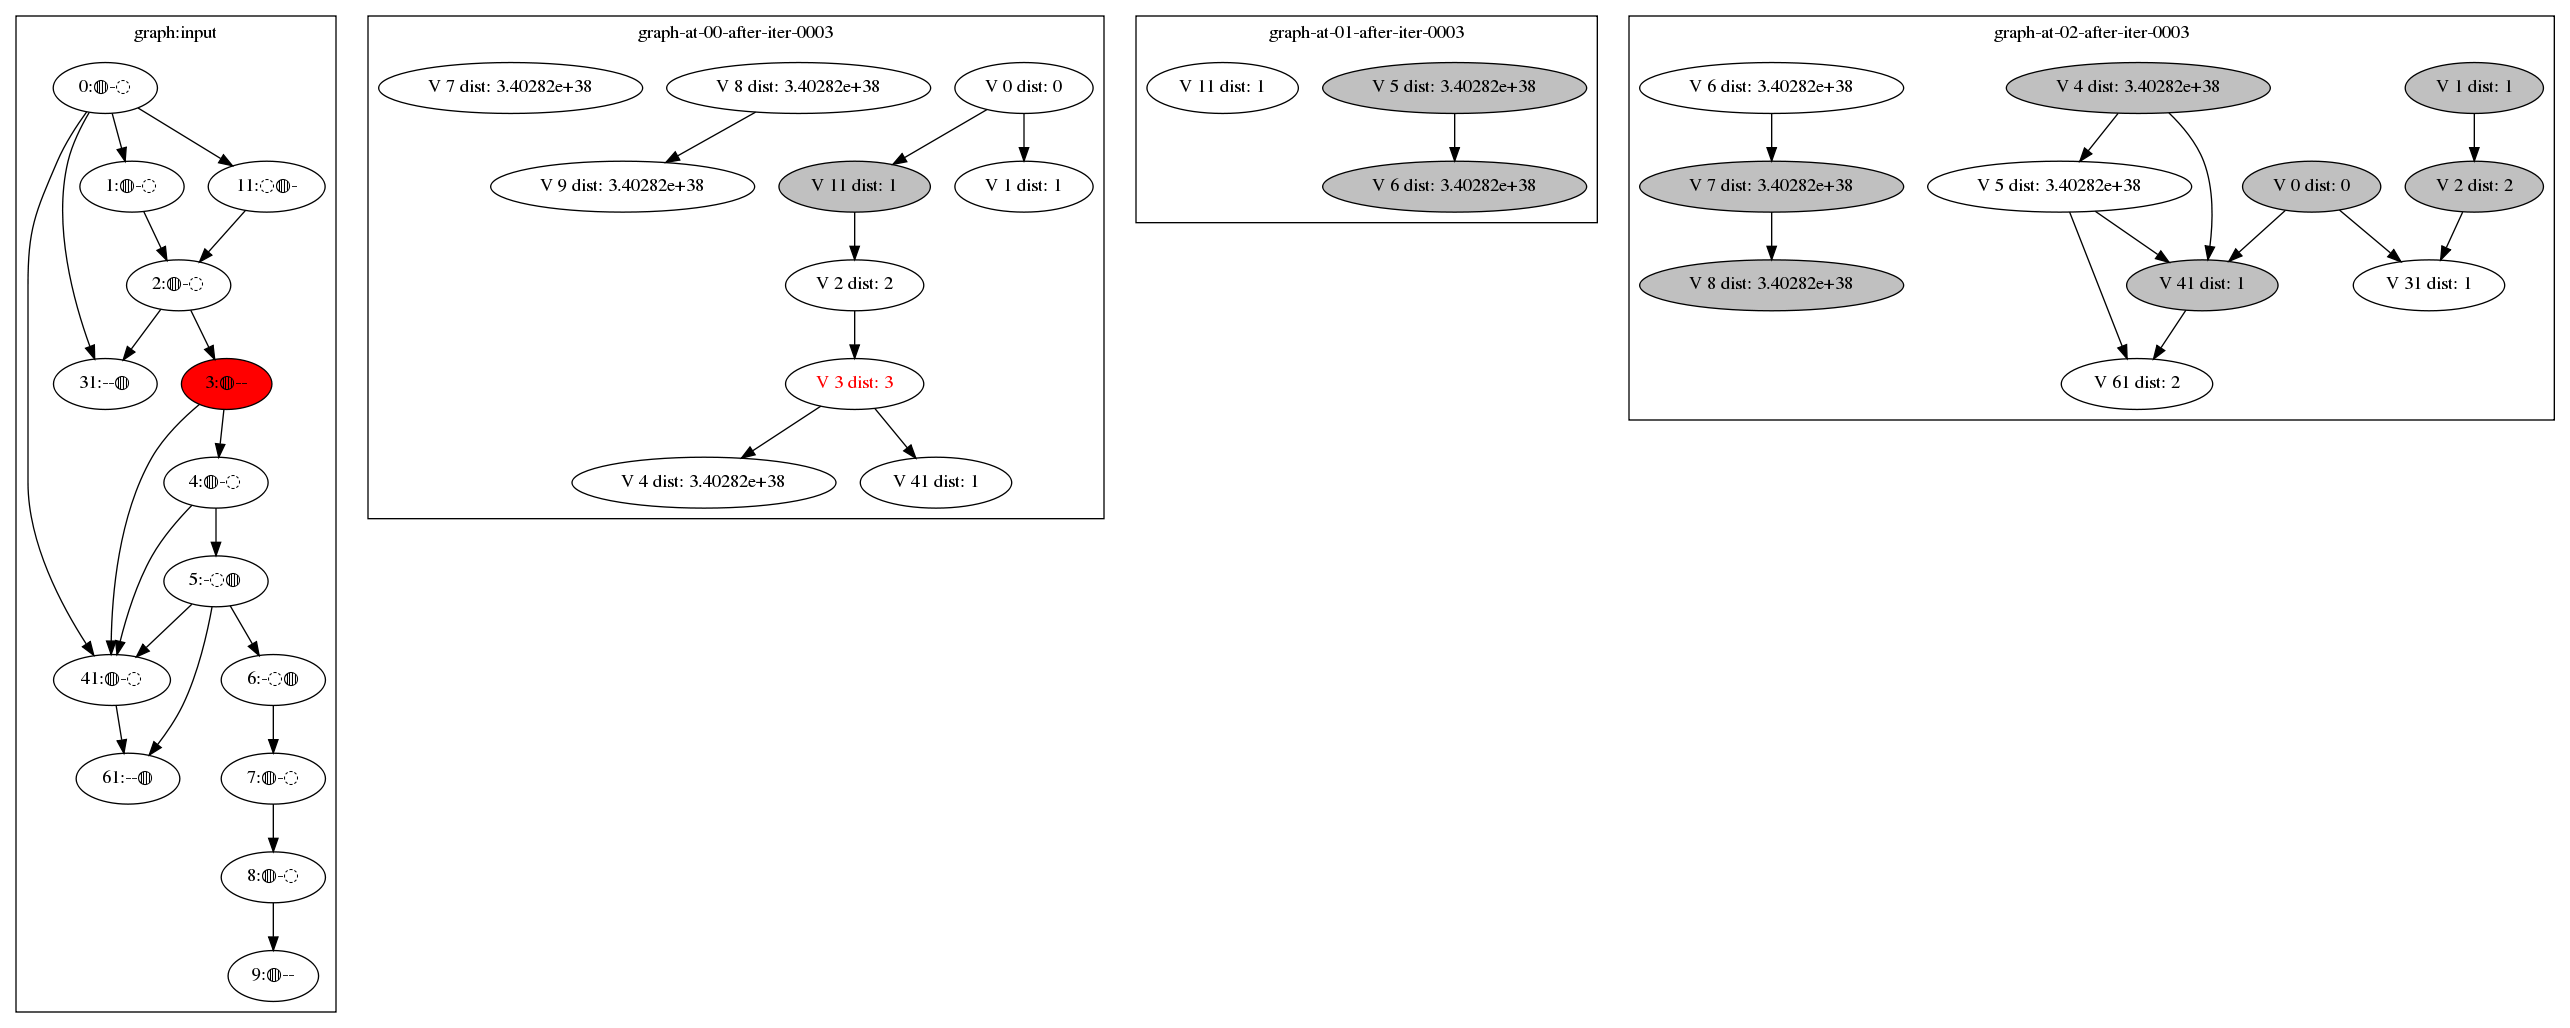
\includegraphics[width=0.8\textwidth]{sync-iter3.png}    
  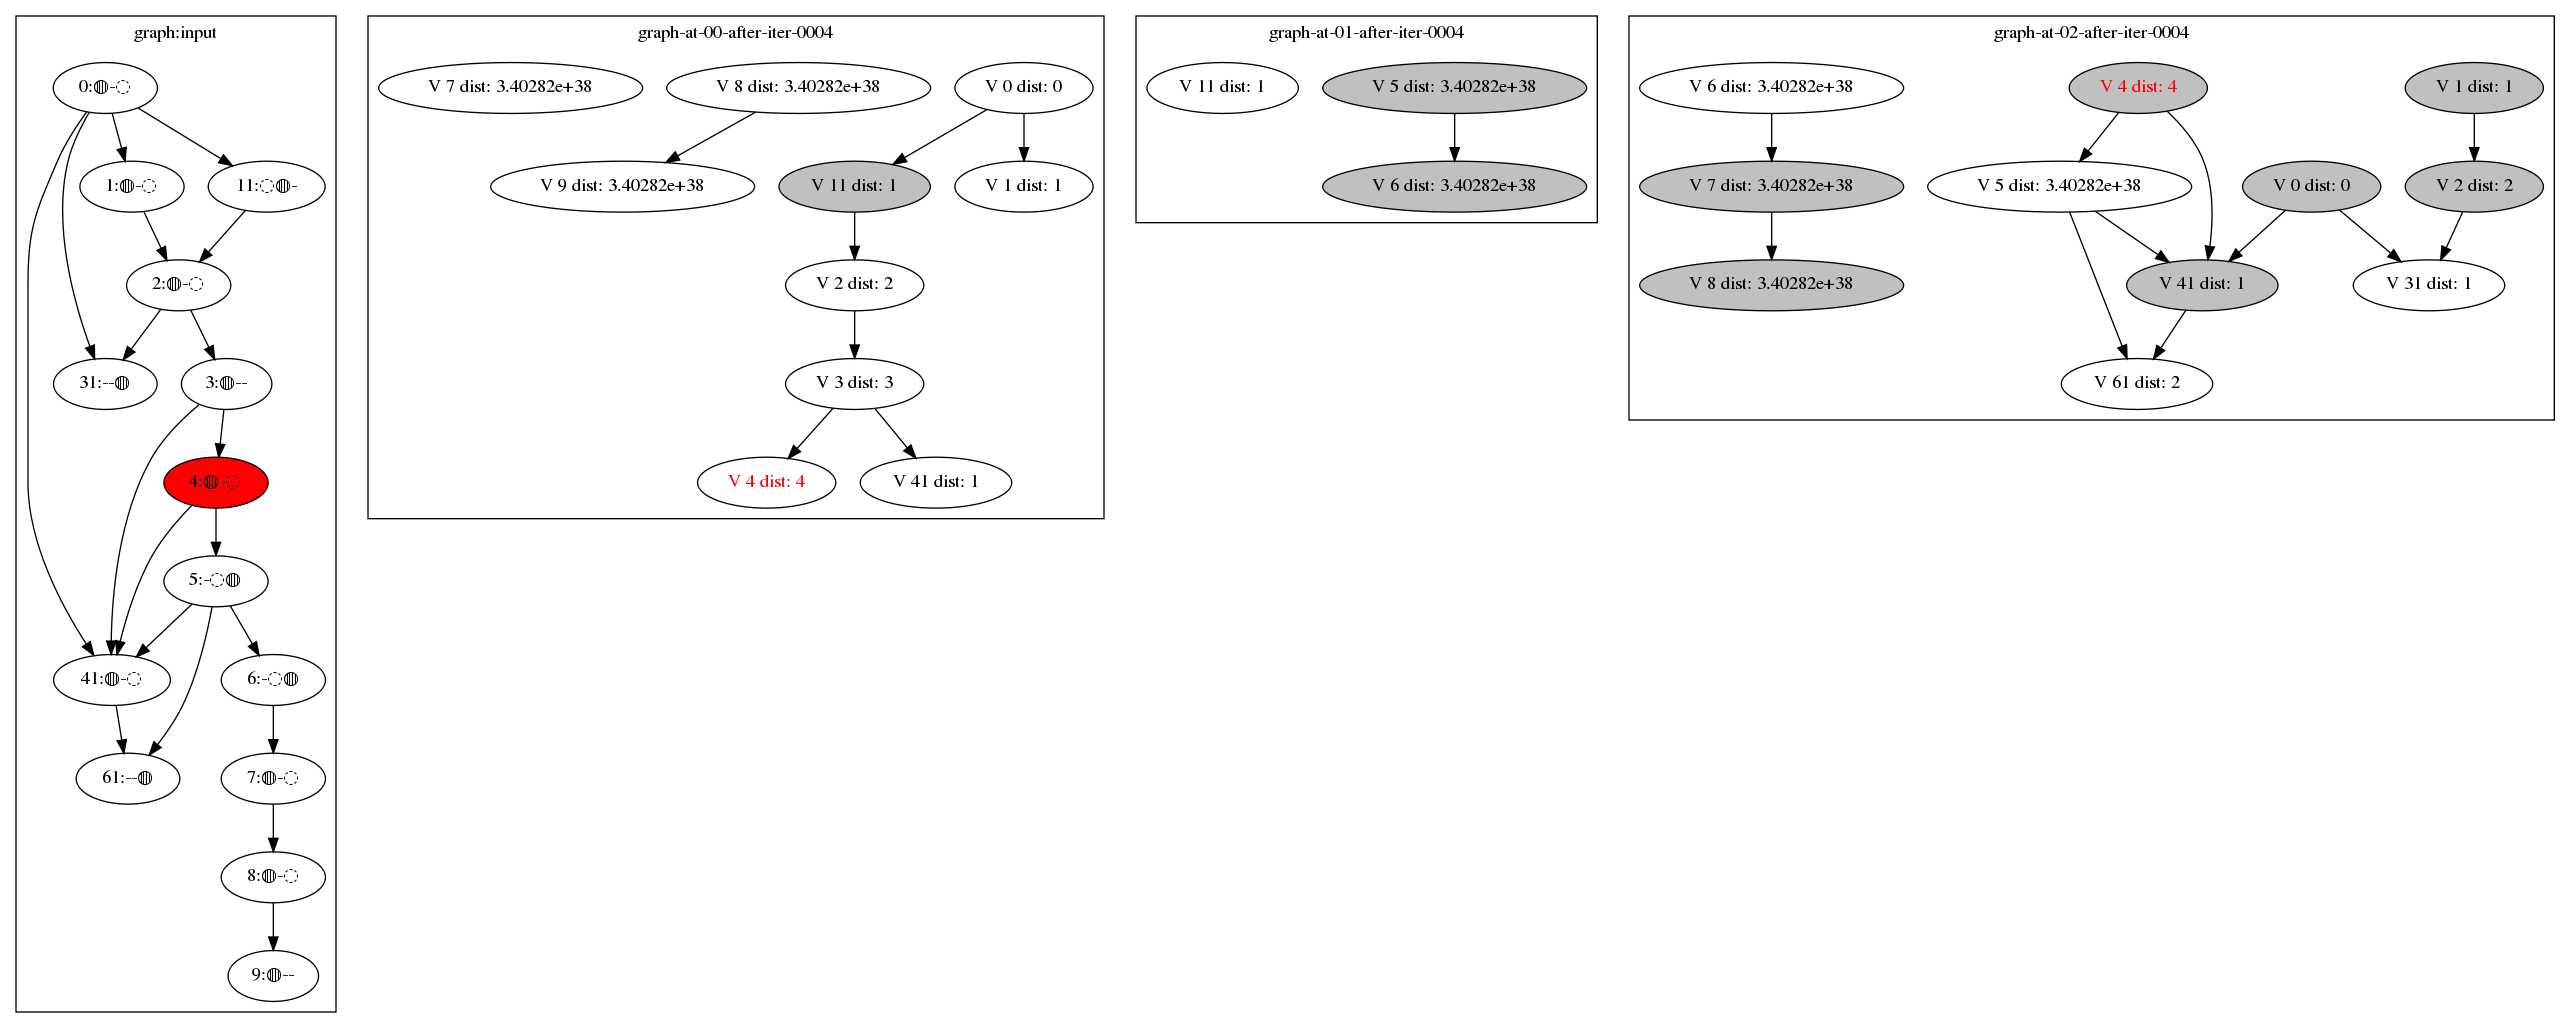
\includegraphics[width=0.8\textwidth]{sync-iter4.png}    
  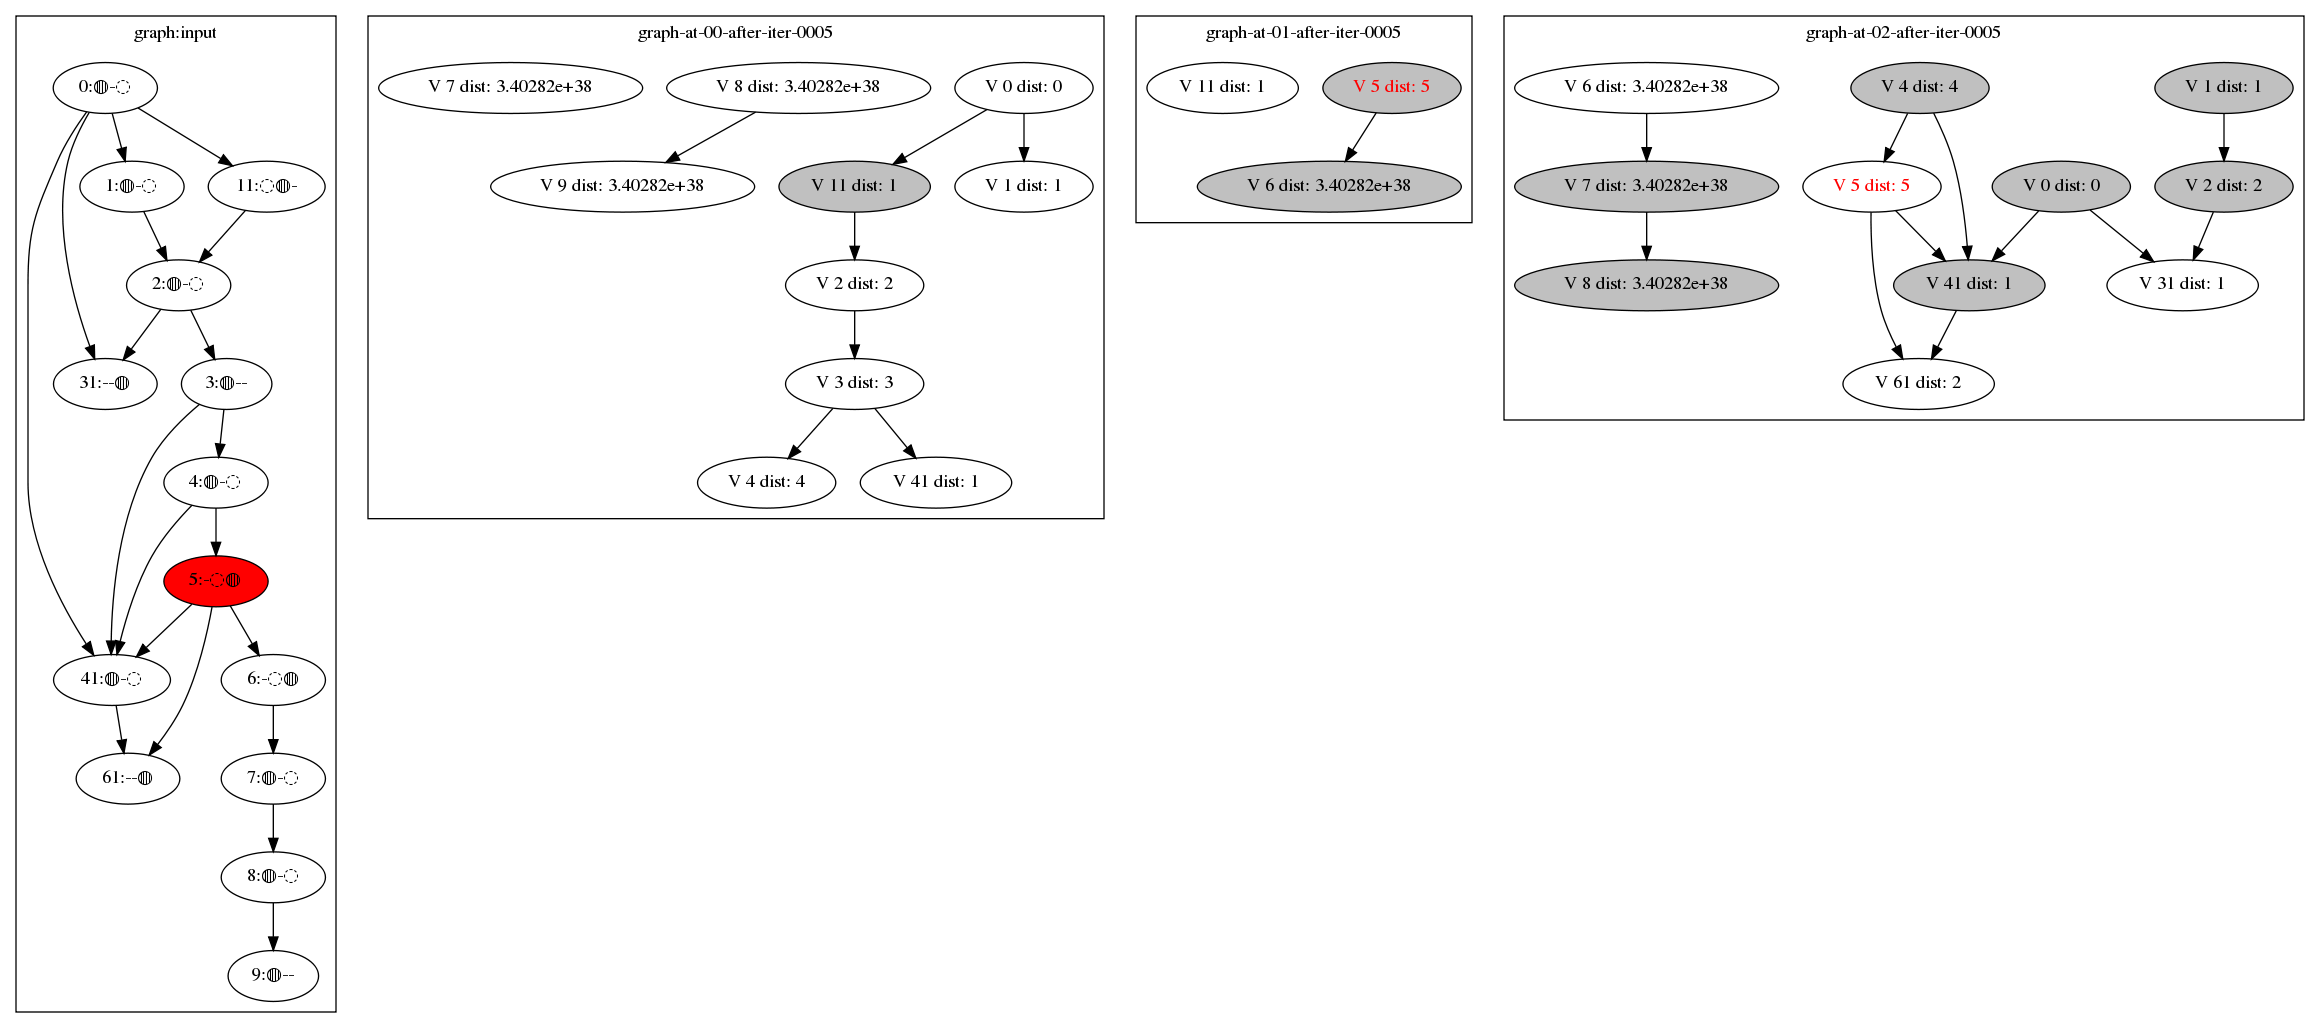
\includegraphics[width=0.8\textwidth]{sync-iter5.png}    

  \captionof{figure}{SSSP算法的迭代过程}
  \label{fig:sssp-sync-iter}
\end{center}  

\subsubsection{开启延迟数据一致性之后的SSSP算法}

开启延迟一致性之后,SSSP算法能够以更少的迭代次数得到同样的结果。
我们以同样的输入图来说明这一点,同时直观的展示延迟数据一致性的具体原理。

\begin{center}
  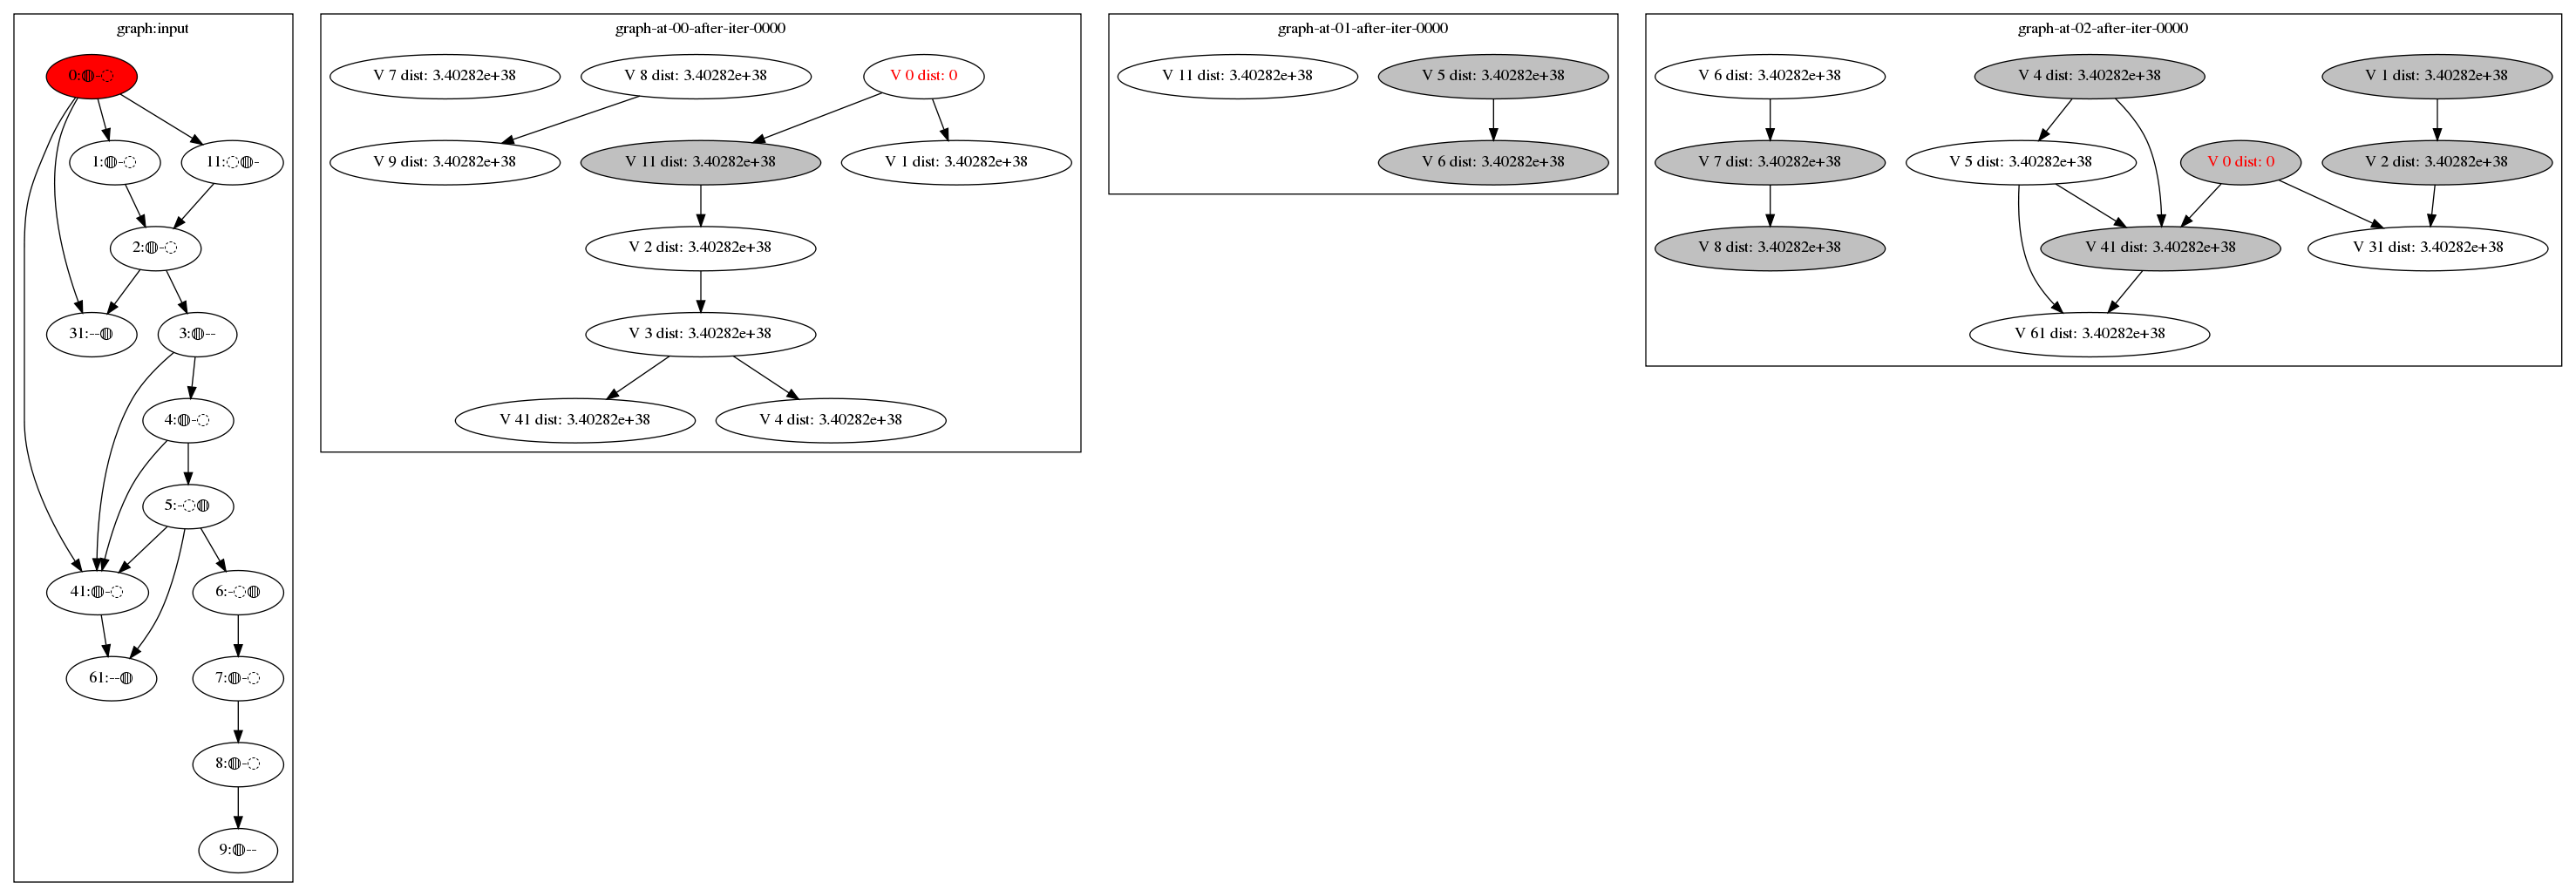
\includegraphics[width=0.8\textwidth]{lazy-iter0.png}
  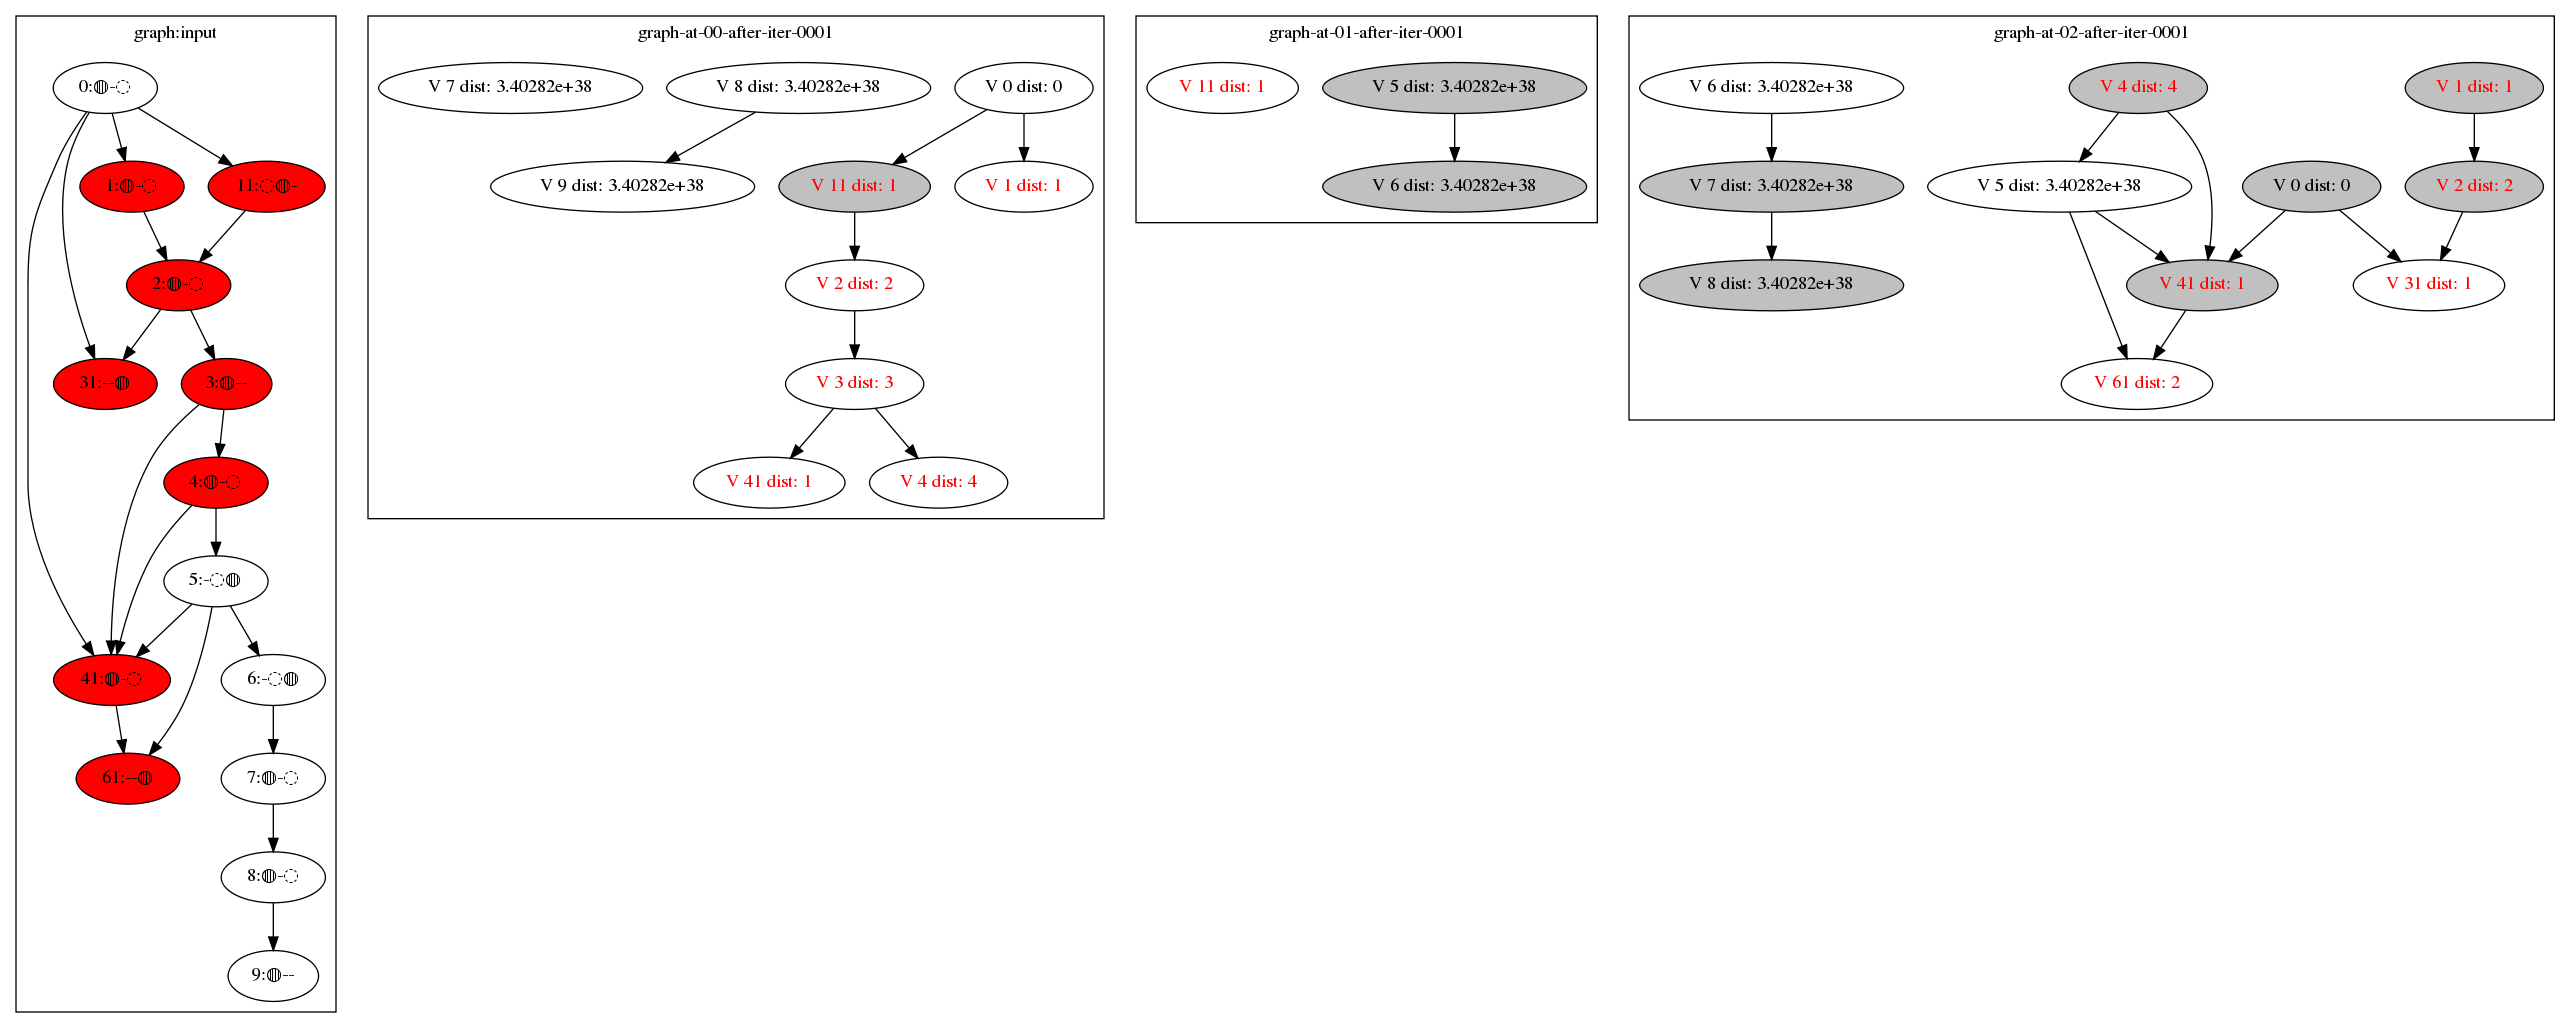
\includegraphics[width=0.8\textwidth]{lazy-iter1.png}
  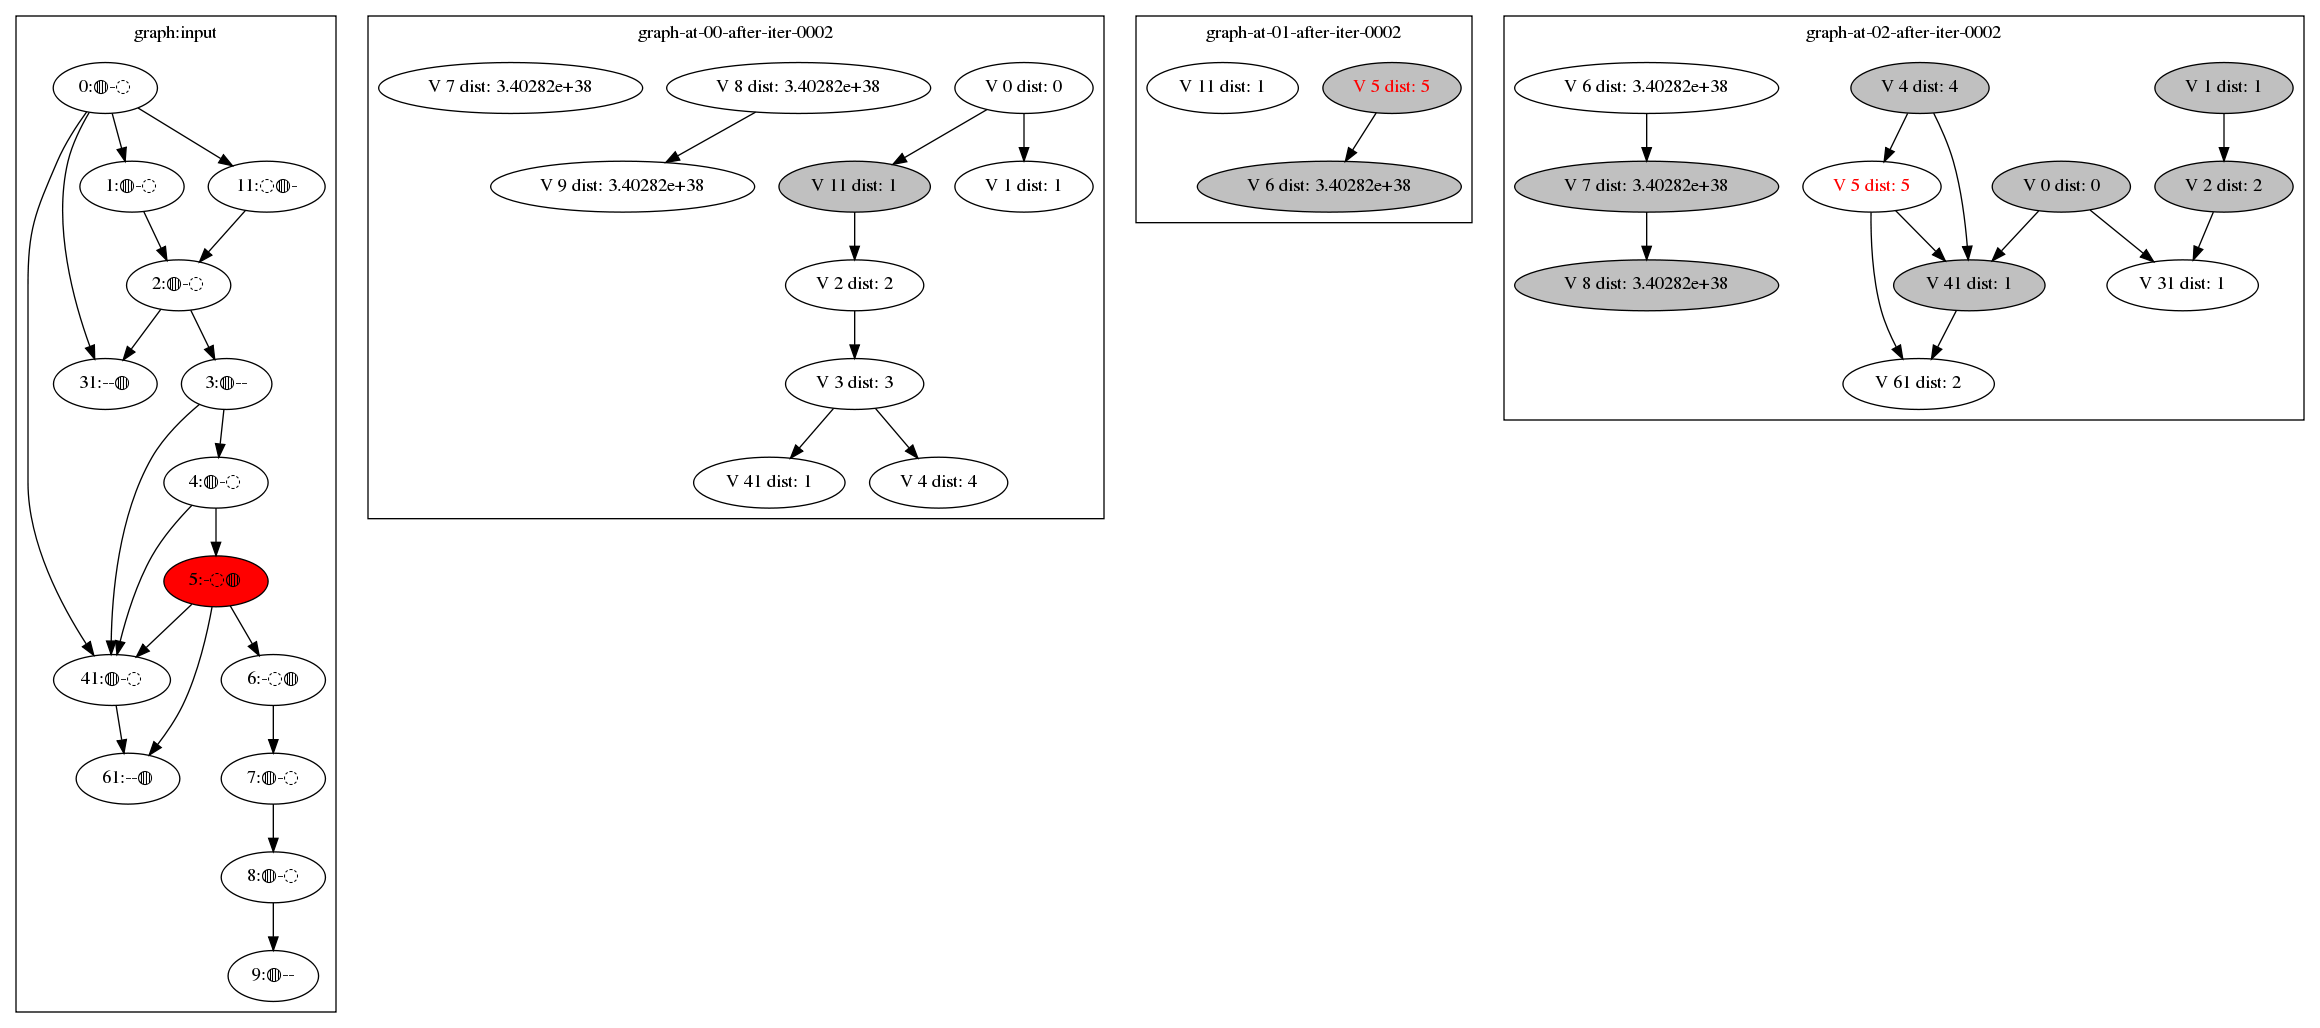
\includegraphics[width=0.8\textwidth]{lazy-iter2.png}    
  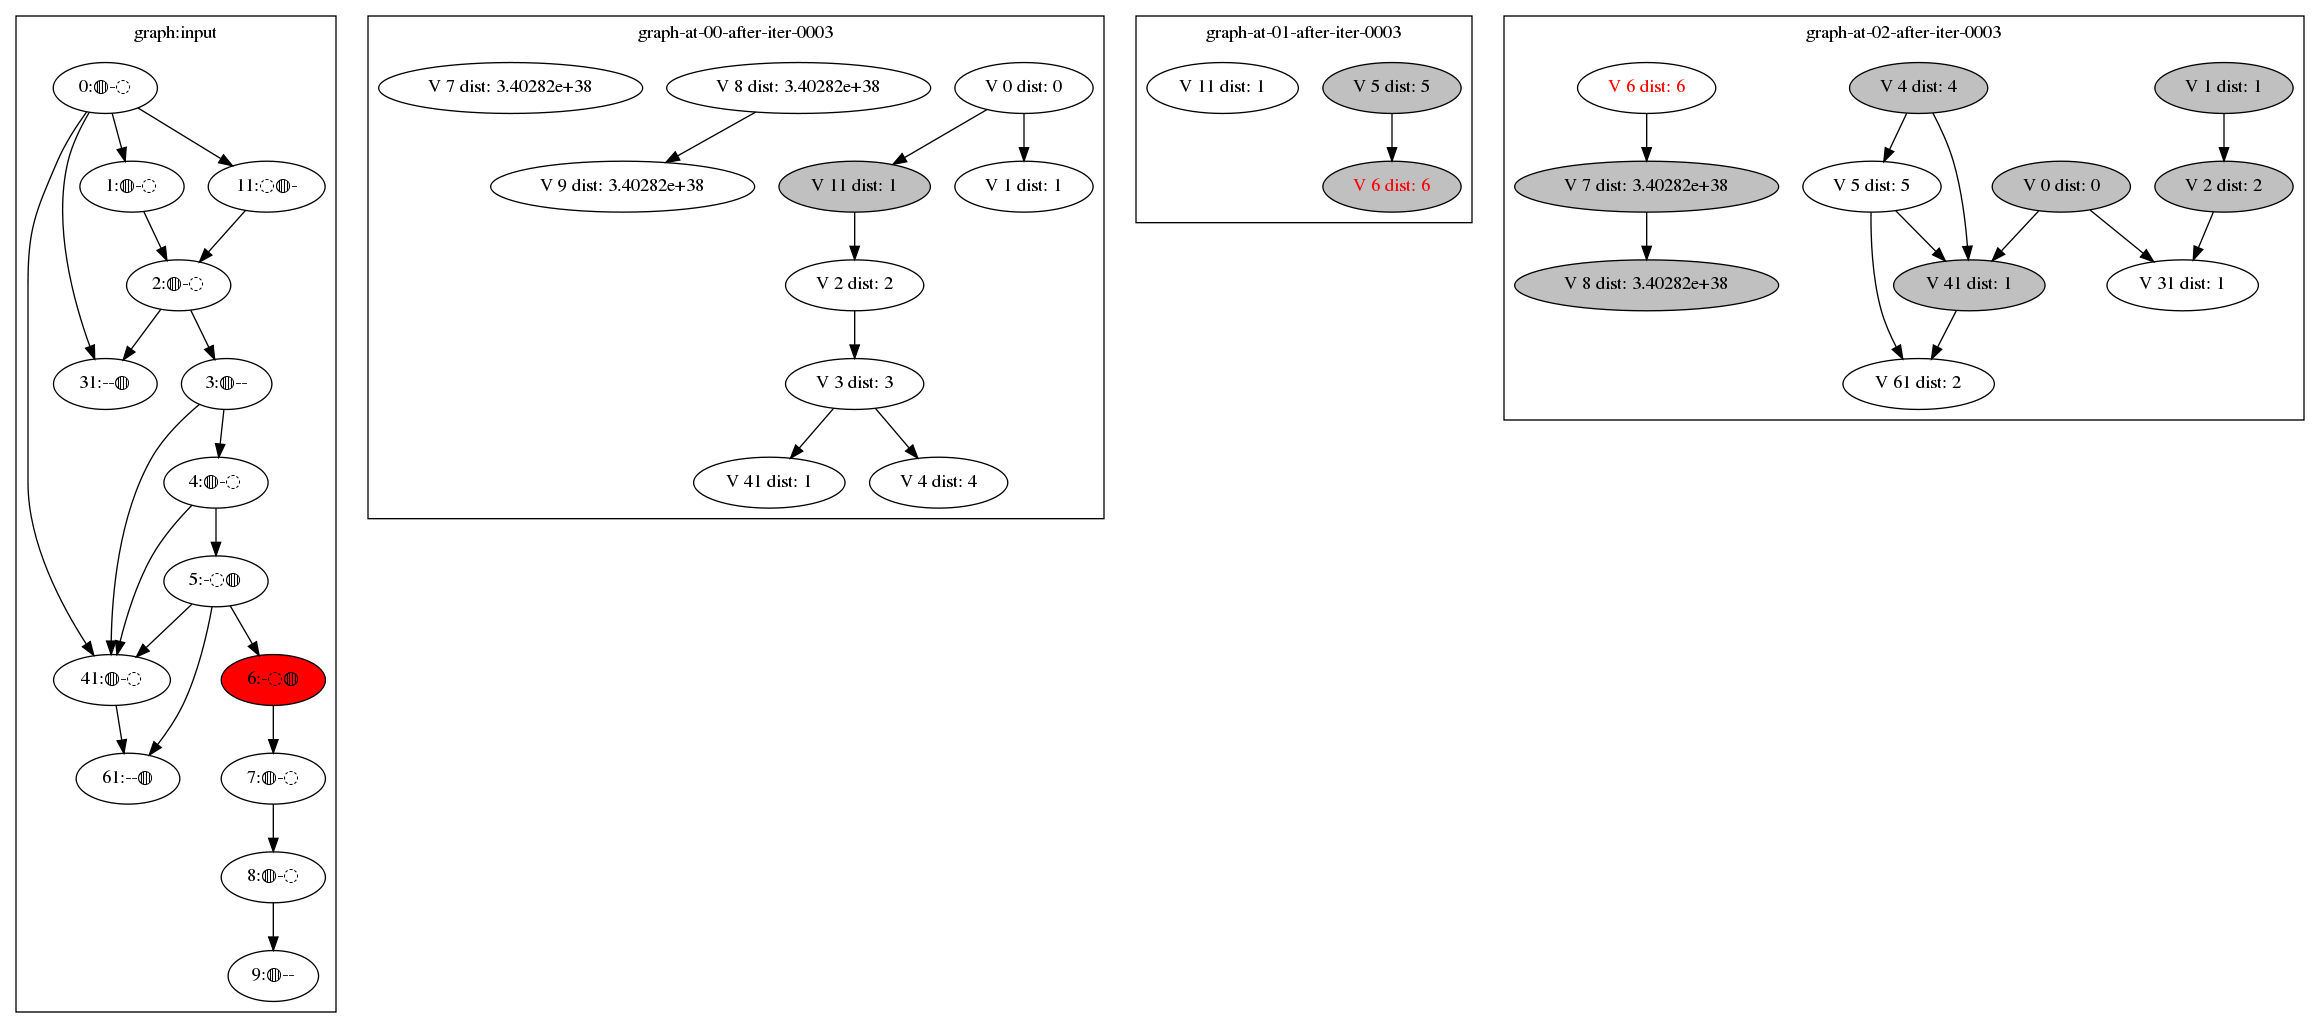
\includegraphics[width=0.8\textwidth]{lazy-iter3.png}    
  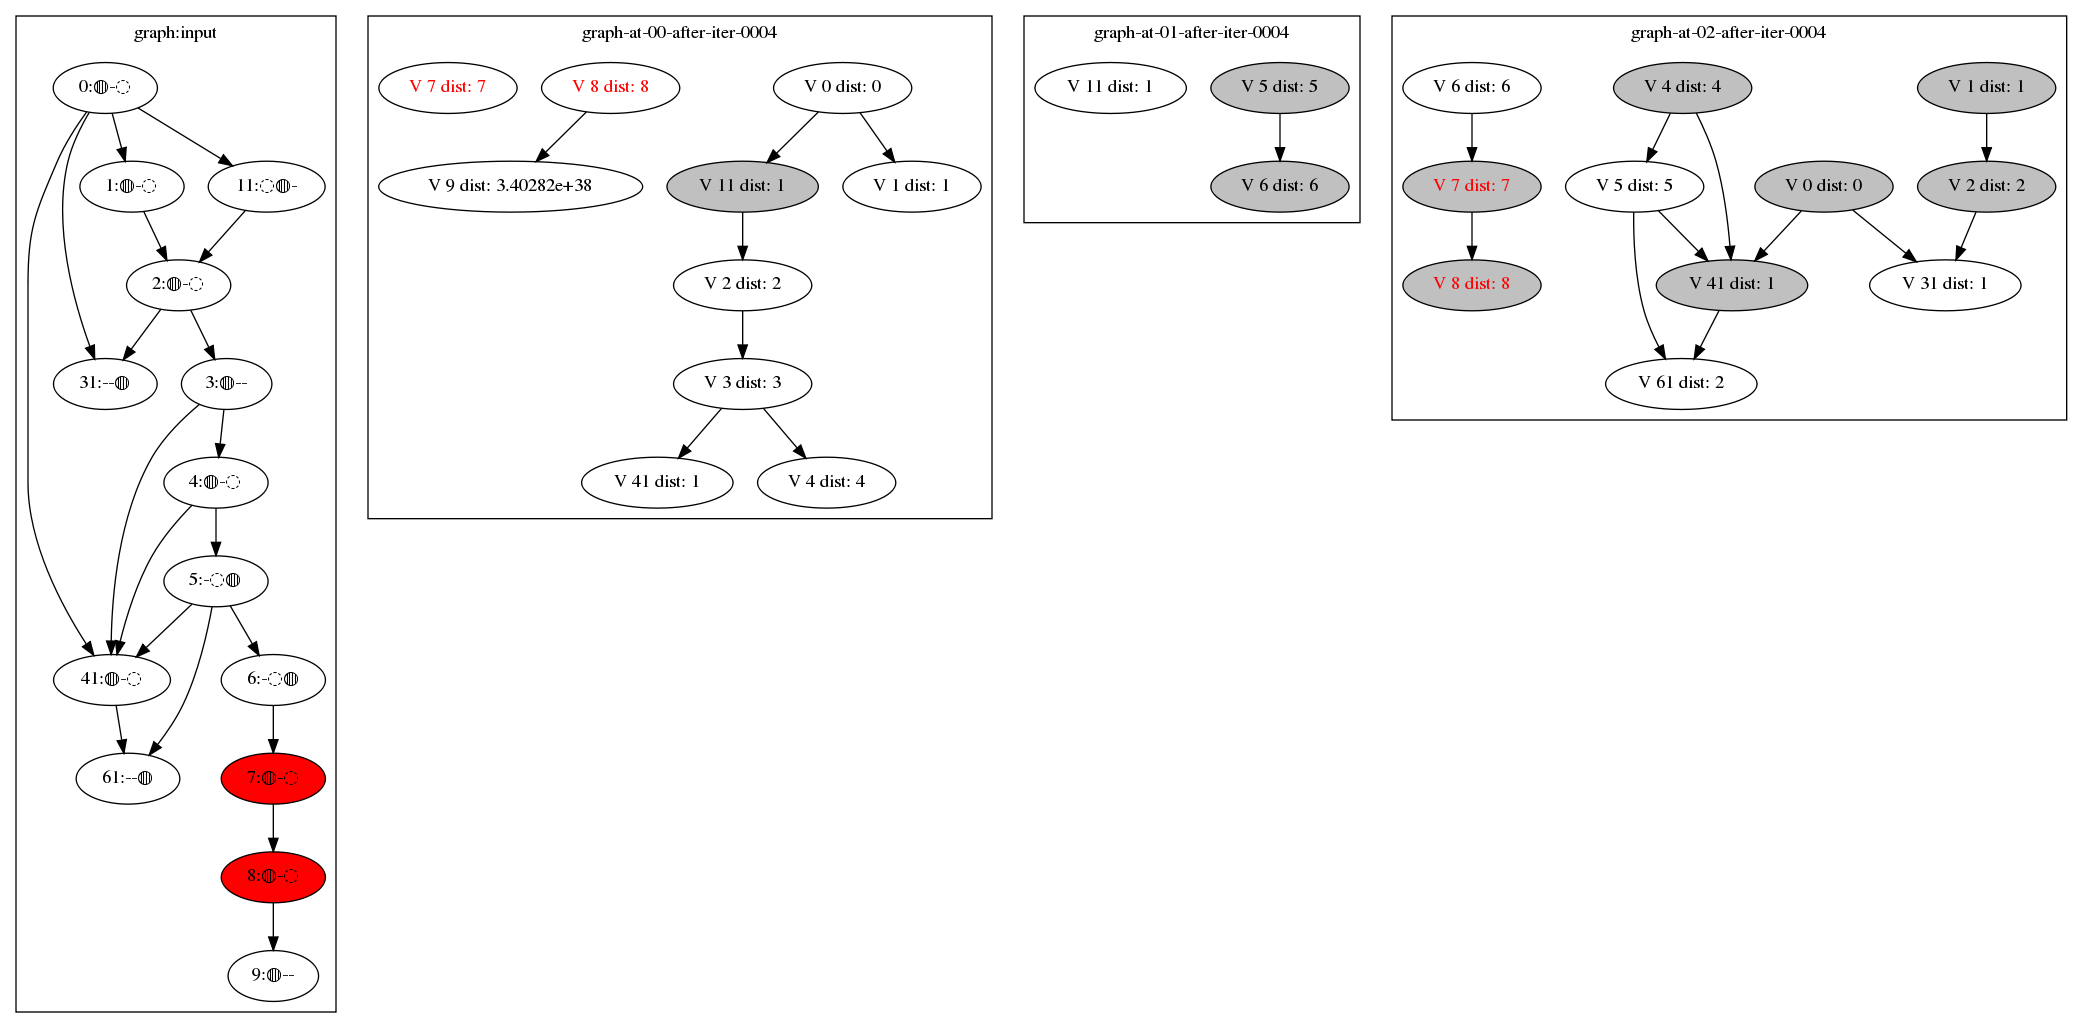
\includegraphics[width=0.8\textwidth]{lazy-iter4.png}    
  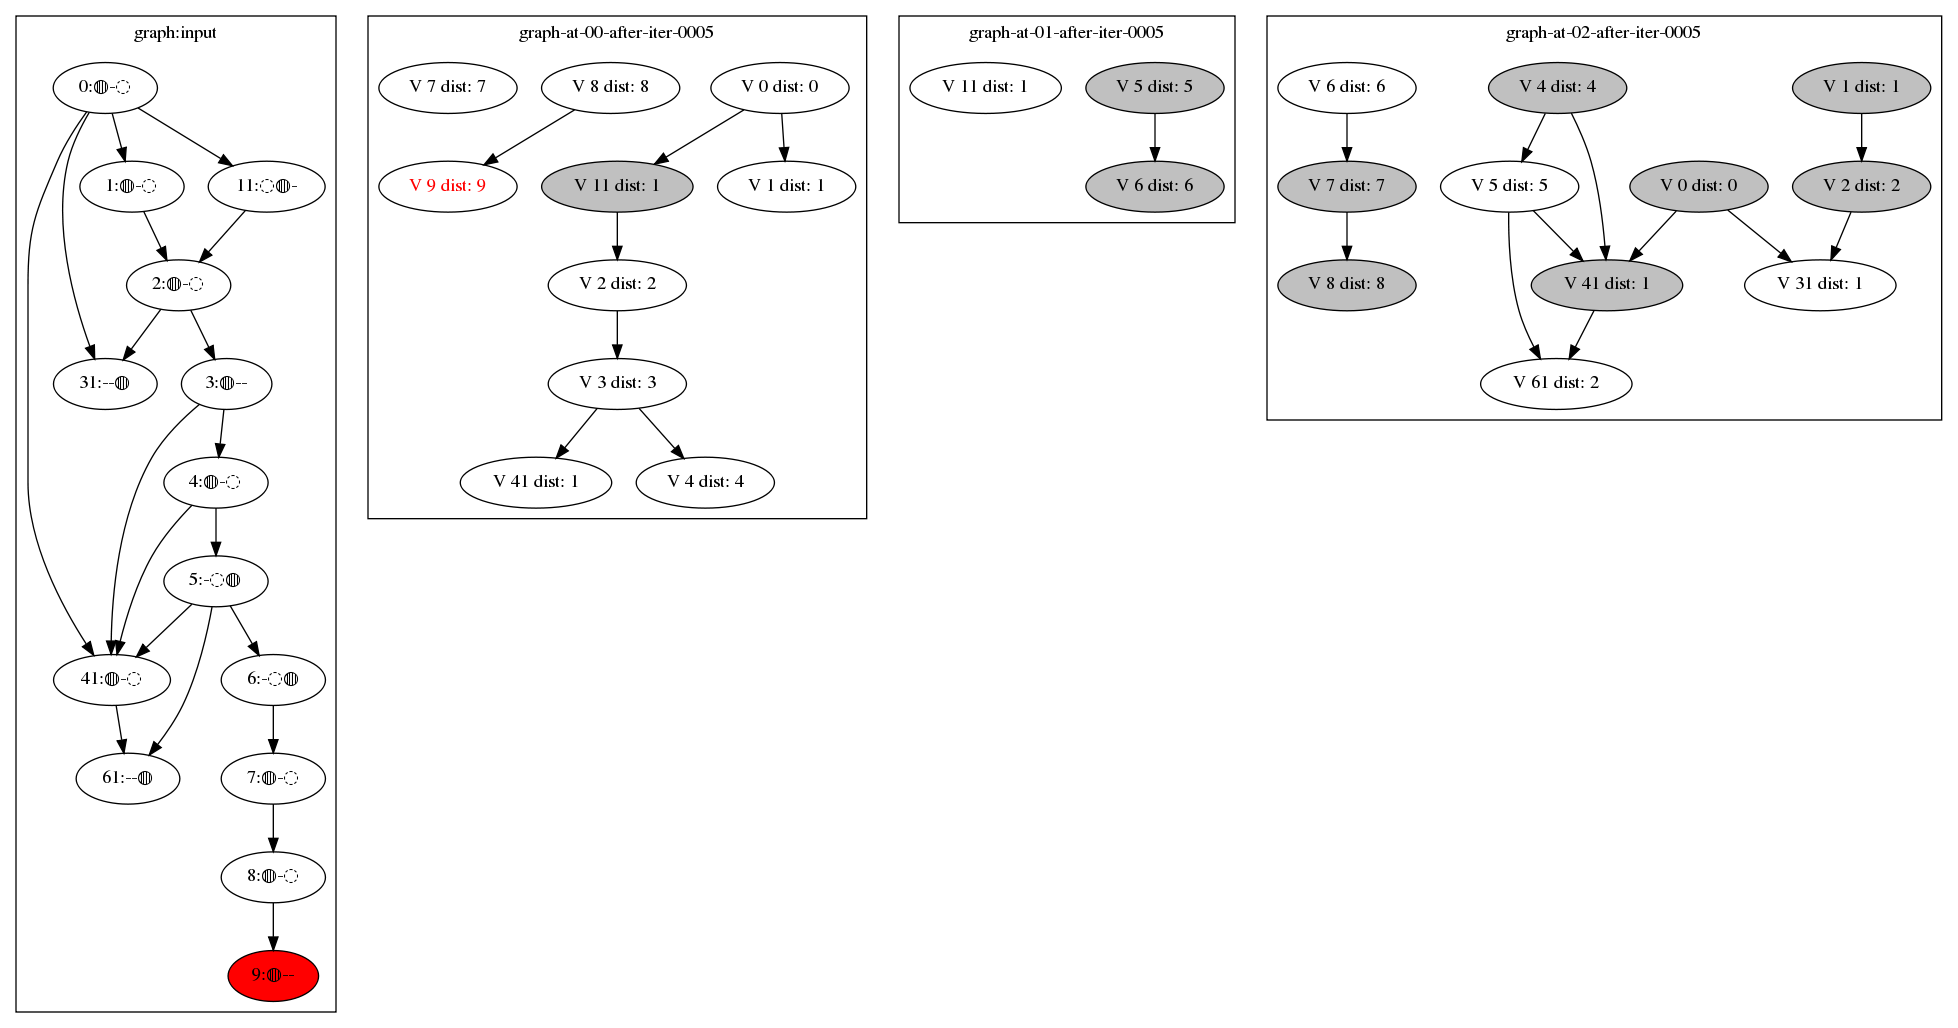
\includegraphics[width=0.8\textwidth]{lazy-iter5.png}
  \captionof{figure}{开启延迟一致性之后SSSP算法的迭代过程}
  \label{fig:sssp-lazy-iter}
\end{center}  


图\ref{fig:sssp-lazy-iter}具体展示了开启延迟一致性之后,SSSP算法的迭代运行过程。
还是同样一个由14个顶点和19条边构成的小图,在3台机器上得到划分结果也是一样的,
以0号顶点为source,计算其他顶点到source的最短距离。
一开始和原始的方式一样,系统会把消息值0发送给0号顶点,进而激活0号顶点,把0号顶点作为活跃点参与计算。  
所以第0轮迭代是一样的,机器0上的master 0 激活了自己的本地邻居 master 1 和 mirror 11,
机器2上的mirror 0 激活了自己的本地邻居mirror 41 和 mirror 31。

但是采用了延迟一致性之后,从第1轮开始,系统的处理方式就和原来的方式产生了不同。
在原来的同步引擎中,系统会先收发消息,然后在master上更新顶点数据。
而在延迟一致性方法中,每次进入新的一轮迭代,系统会先进行本地计算。
在本地计算中,每台机器会先根据自己的本地消息进行互相独立的计算,同时会把本地计算过程中的消息累加起来。

反映在图中,进入第1轮迭代时,
在机器0上存在着上一轮master 0发送给master 1 和 mirror 11的消息,那么本地计算会根据这两个消息把1号顶点和11号顶点
作为活跃点立即进行GAS迭代计算,而mirror 11则会进一步激活它的本地邻居master 2,
然后master 2进一步激活它的本地邻居master 3, 然后 master 3进一步激活它的本地邻居master 41 和 master 4,
而master 1则由于没有本地邻居而不会进一步激活,
这样机器0上不需等待和消息交换经过本地计算之后就已经激活并计算了mirror 11, master 1, 2,3, 4, 41这 6个顶点,
并且此时求得它们顶点上的值分别为1,1,2,2,3,4,4;
在机器1上由于不存在本地消息,也就没有本地计算的过程;
在机器2上存在着上一轮mirror 0发送给master 31 和 mirror 41的消息,那么本地计算会根据这两个消息把41号顶点和31号顶点
作为活跃点立即进行GAS迭代计算,而mirror 41则进一步激活它的本地邻居master 61,而master 31由于没有本地邻居不会进一步激活,
这样机器2上在本地计算阶段激活了mirror 41, master 31, 61,并且此时求得它们顶点上的值分别为1,1,2。

在所有机器上的本地计算都完成之后,系统进入到了数据一致性阶段。
在数据一致性阶段,本地计算中被激活的点都要参与计算进行数据一致。
数据一致性阶段会先对各个活跃点在本地计算期间得到的消息累加和进行交换,
然后活跃点的master部分和mirror部分按收到的消息进行各自进行一轮独立的GAS计算。
在数据一致性中经过apply部分之后,活跃点的master部分和mirror部分经过计算实现数据一致,
然后活跃点的master和mirror部分会各自进行scatter部分激活自己的本地邻居,让系统进入下一轮迭代。
反映在图中,我们注意到,经过本地计算除了11,1,31,41之外,系统额外激活并计算了2,3,4,61,并且计算的结果都是准确的。

这里需要注意到,机器0上对master 41进行本地计算得到的是4,而机器2上对mirror41进行本地计算得到的是1,而1才是41号顶点上的正确结果。
显然本地计算之后,正确结果出现在哪个副本上是不确定的,延迟一致性方法是怎样自动得到了正确的结果呢? 
正是依靠交换本地计算阶段的累加和,使得数据一致性阶段之后,活跃点的master部分和mirror部分上求得的值都是一样的。
这里,机器上0上master 41交换到了机器2上mirror 41记录的本地累加和1从而最终也求得了正确结果1。

第1轮迭代经过本地计算阶段和数据一致性阶段之后,系统进入了第2轮迭代。
在第1轮的数据一致性的scatter计算中,机器0和机器1上的活跃点都没有额外激活本地邻居,因为没有本地消息的产生,
只有机器2上mirror 4激活了本地邻居master 5。
所以在第2轮迭代的本地计算阶段,只有机器2上有本地消息,也就只有机器2进行本地计算。
机器2上的本地计算处理玩本地消息后激活并计算了master 5上的值是5,然后本地计算也由于没有需要激活的本地邻居而结束。
在第2轮迭代的数据一致性阶段,mastr 5和mirror5通过消息交换得到了同样的全局视图。

5号顶点进一步激活6号顶点作为第3轮的活跃点,直到最后系统总计经过6轮迭代之后没有活跃点趋于收敛。
这样,对于同样的输入图,同步引擎需要10轮迭代,而延迟一致性方法只用6轮迭代就能得到同样的正确结果。



以上述这个小图为例,我们在展示延迟一致性方法的原理的同时,
也看到了这种方法是如何提高图计算效率的。
我们看到 LazyAsync 方法之所以能够减少全局迭代次数是因为
这种方法的本地计算中额外进行了多轮激活迭代。
在同步引擎中,每次迭代之后要进行数据同步和屏障等待才能进入下一轮迭代。
而在延迟一致性方法中,活跃点的更新是在本地立即可见的,并且这个更新会进一步的激活更多本地活跃点进行计算。
同时由于计算是在本地进行的,不存在网络中的数据交换,读写都是在本地内存中进行,使得本地计算效率更高。
所以这种延迟一致性方法相当于在同步引擎中引入了异步引擎的语义\cite{Ju@MACS17},同时又不用像异步引擎那样加全局加锁来维护数据一致\cite{Xie@PPoPP15}。

由于本地计算中更新立即可见并在本地继续传播使得很多活跃点提前收敛,延迟一致性方法往往能减少图计算的全局迭代次数,降低计算时间。
以一个来自snap\cite{SNAP}数据集的大图road-USA-net为例,这是一个包含 2400 万个顶点和5800万条边的大图,
在48机的集群中,采用原始的 eager data coherency 方法,对这个图完成 SSSP 计算需要5610轮迭代,耗时1083 s, 
使用 lazy data coherency 方法之后,只需要1604轮迭代,耗时176s,
LazyAsync 带来了6倍的加速比。

但是延迟数据一致性方法在某些情况下虽然减少了迭代次数却并没有带来时间上的性能收益。
这一点从总计算时间的构成公式\cite{bsp@1990}中也可以理解:$T=iter \times t_{per\_iter}$。
总时间由$iter$ 和 $t_{per\_iter}$共同影响,如果 $iter$ 减少的同时,$t_{per\_iter}$增大了,
那么总时间就并不一定会减少,甚至会增大。
延迟一致性方法能够解释并保证迭代次数的减少,但它对平均每次迭代时间的影响却是不一定的。
所以延迟一致方法需要合适的开启策略才能在减少迭代次数的同时,也保证不增加甚至减少平均每次迭代时间
这样最终才能得到相对最优的性能提升。

\subsection{冗余计算带来性能损耗}
仍以SSSP为例,本文继续研究了延迟一致性方法对平均每次迭代时间的影响。
最终发现,LazyAsync 方法虽然避免了 eager data coherence 方法中存在的冗余的同步,等待及通信,
\textbf{但是这种方法却有可能在本地计算过程中引入新的冗余计算}。
本地计算过程中的冗余计算会增加单次迭代计算时间,这样一来LazyAsync方法虽然减少了图计算过程的迭代轮次,
但是却最终因为单次迭代时间的增加而拿不到相对最优的性能提升。


在图\ref{fig:sssp-lazy-iter}中,每一轮迭代之后本地计算激活的点在数据一致性阶段最终都求得了正确的值。
所以,每次迭代中的本地计算部分带来的都是性能收益。
然而这只是最理想的情况,实际中考虑到输入图和划分的多样性,
完全存在另一种可能\textbf{使得本地计算中的大部分计算是无效的,
进而使得本地计算带来的是性能损失,最终使得延迟一致方法并不能带来性能收益}。
我们仍以一个小图来说明这种情况。


图\ref{fig:useless}具体展示了延迟一致性方法的一次迭代中存在的有效计算与无效(冗余)计算的情况。
在图\ref{fig:useless}中,最左边是一个完整的输入图,右边是这个图划分到2台机器上的情况。
这个划分并不均衡,它是为了演示本地计算中存在的有效计算与无效计算而特意构造的。
但是在实际的图计算中,作为一个子图,这种划分结果是完全可能存在的,
因而这里所演示的情况也是实际会发生的。

在图\ref{fig:useless}中,机器0上的0号顶点收到了本地消息,按照延迟一致方法中的本地计算的原则,
机器0上的0号顶点会进一步把本地子图中的连通邻居进一步激活,而机器1上由于没有本地消息则没有进行本地计算。
机器0上本地计算之后,对顶点1,2,21,22,23的计算都是正确有效的,但是对于顶点3,4,5,6,7,8的计算都是错误因而无效的。
并且,其中4,5,6,7,8号顶点的计算无效都是因为对3号顶点的计算无效造成的。
而对3号顶点的无效计算是因为从1号顶点到3号顶点有一条更短的路径,使得3号顶点上的值应为2,
但是由于1-3这条边不在本地,使得本地对计算中对3号顶点的计算是错误的,从而后续的一系列计算都成了无效计算。
最终,在机器0的本地计算中激活了11个顶点,但是只有5个顶点上的计算是有效的,其他6个顶点上的计算是无效的。
这样延迟一致方法的本地计算额外多计算了4个点是正确的,但同时也额外多算了6个点是无效的。
这种情况下,延迟一致方法虽然还是能够减少迭代次数,但在本次迭代中执行了不必要的冗余计算,
最终并不能保证得到很好的性能收益。

\begin{center}
  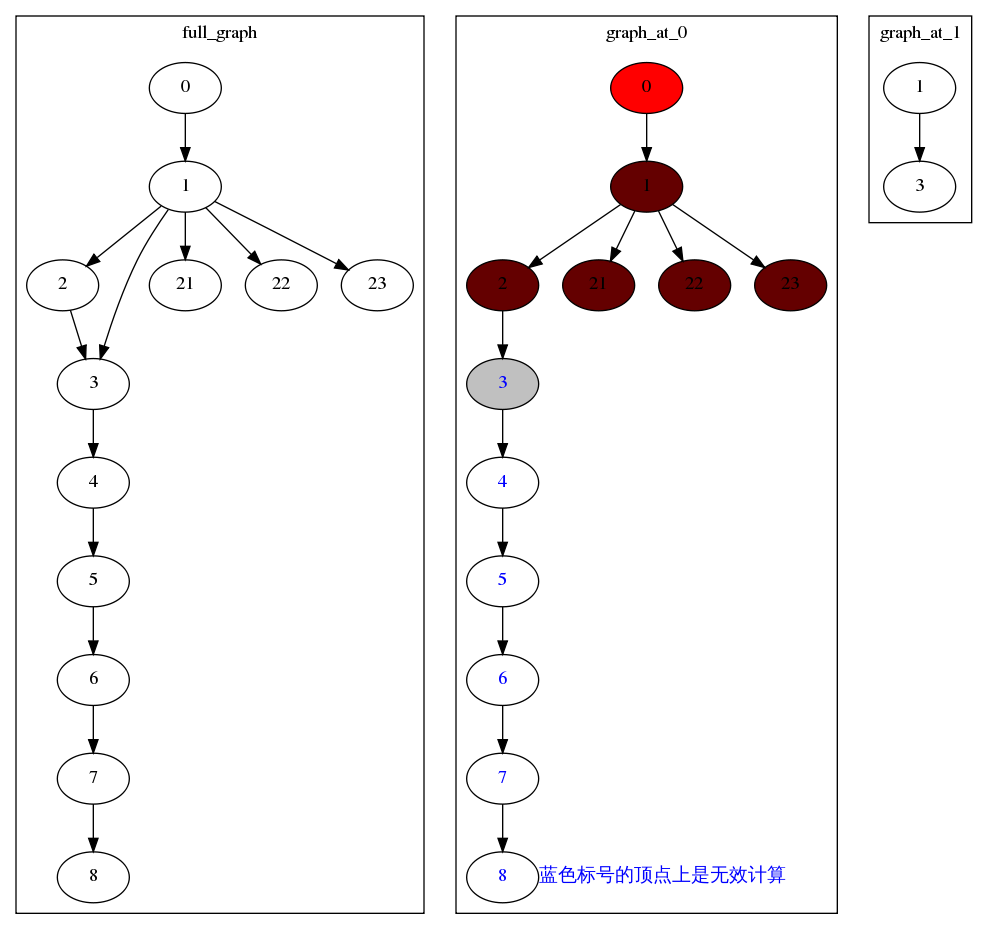
\includegraphics[width=0.8\textwidth]{useless.png}
  \captionof{figure}{有效计算与无效计算示意图}
  \label{fig:useless}
\end{center}  

这里需要额外说明,本地计算中的错误计算最终会被纠正,不会影响最终结果的正确性。
在图\ref{fig:useless}中,本地计算之后,顶点3,4,5,6,7,8上计算的当前值并不等于计算收敛时的正确值。
这在迭代计算中是完全合理的。
并且在本轮数据一致之后,机器1上的master 1会得到机器0上的mirror 1的正确视图,进而激活master 3。
这样,master 3就在后来的迭代中求得了正确值,并进而正确的激活它的后续邻居,
最终延迟一致方法还是能够求得正确结果。

经过以上的分析,我们可以发现,延迟一致性方法能够减少图计算的迭代轮次,提高图计算的计算效率。
但是这种效率的提高受每轮迭代中本地计算的有效程度的影响而不同。
延迟一致方法的性能提升来自于它的本地计算能够在本地传播多轮更新值,提前对更多的本地连通点进行计算。
但是,如果本地计算中某些顶点上的值计算错误,那么这些点引起的后续计算都将是错误而无效的
(虽然这些错误最终会在后边的迭代中被纠正)。
这样本地计算带来的就是额外的不必要的性能损失。


\section{通过比较迭代解和最终解量化LazyAsync 方法的性能收益}  

在上一个小节,我们通过一个小图定性地观察了延迟一致方法性能收益和性能损耗的来源。
为了探究延迟一致方法和它带来的图计算性能提升之间的规律,我们需要对延迟一致方法的性能收益进行量化。
这里我们采用迭代解和最终解的关系来具体量化延迟一致方法的性能收益。

每次迭代之后,活跃点经过本地计算和数据一致都会得到一个迭代解。
同时,在迭代计算结束时,每个点都有一个最终解。
我们通过计算每次迭代结束时有效计算的比例,也就是有多少活跃点的迭代解等于最终解,
来对一次迭代中的延迟一致的收益进行量化。
显然有效计算的比例越高,延迟一致方法的性能收益就越好。
相反,有效计算的比例越低,延迟一致方法的性能收益就越差。
在SSSP算法中,对于同步引擎来说,每次迭代,活跃点经过计算得到的迭代解都等于最终解。
所以,对于同步引擎的SSSP算法来说,有效计算的比例总是为1的。


这其中存在一个问题,最终解是图计算的最终计算结果,是无法事先知道的,只有计算结束时才能得到。
对此,我们让程序先跑一遍把结果存下来,然后再修改程序从结果中读入最终解。
这样每次迭代时,每个顶点都能同时知道它的迭代解和最终解,从而能够比较。
这是为了对延迟一致方法的具体效果进行观察而采用的一种技术手段。



在确定了量化延迟一致方法的有效计算比例的手段之后,我们在一些大图上进行了实验。
在某些本地性比较好的图上,延迟数据一致性方法不需要进行手动调优直接开启就能得到相对最优的提升效果。
所以这里主要对比了SSSP算法在本地性不好需要调优的图上调优前后LazyAsync方法所进行的有效计算的数量和比例。
在本地性不好的图上,立即开启延迟一致无法得到最好的性能提升,开启的太晚也无法得到最好的性能提升。
本文正是要寻找一种自适应优化手段使得LazyAsync方法能够在这类图上自动地得到相对最优的性能提升效果。

\begin{figure}[!htbp]
  \centering
  \begin{subfigure}[b]{0.4\textwidth}
    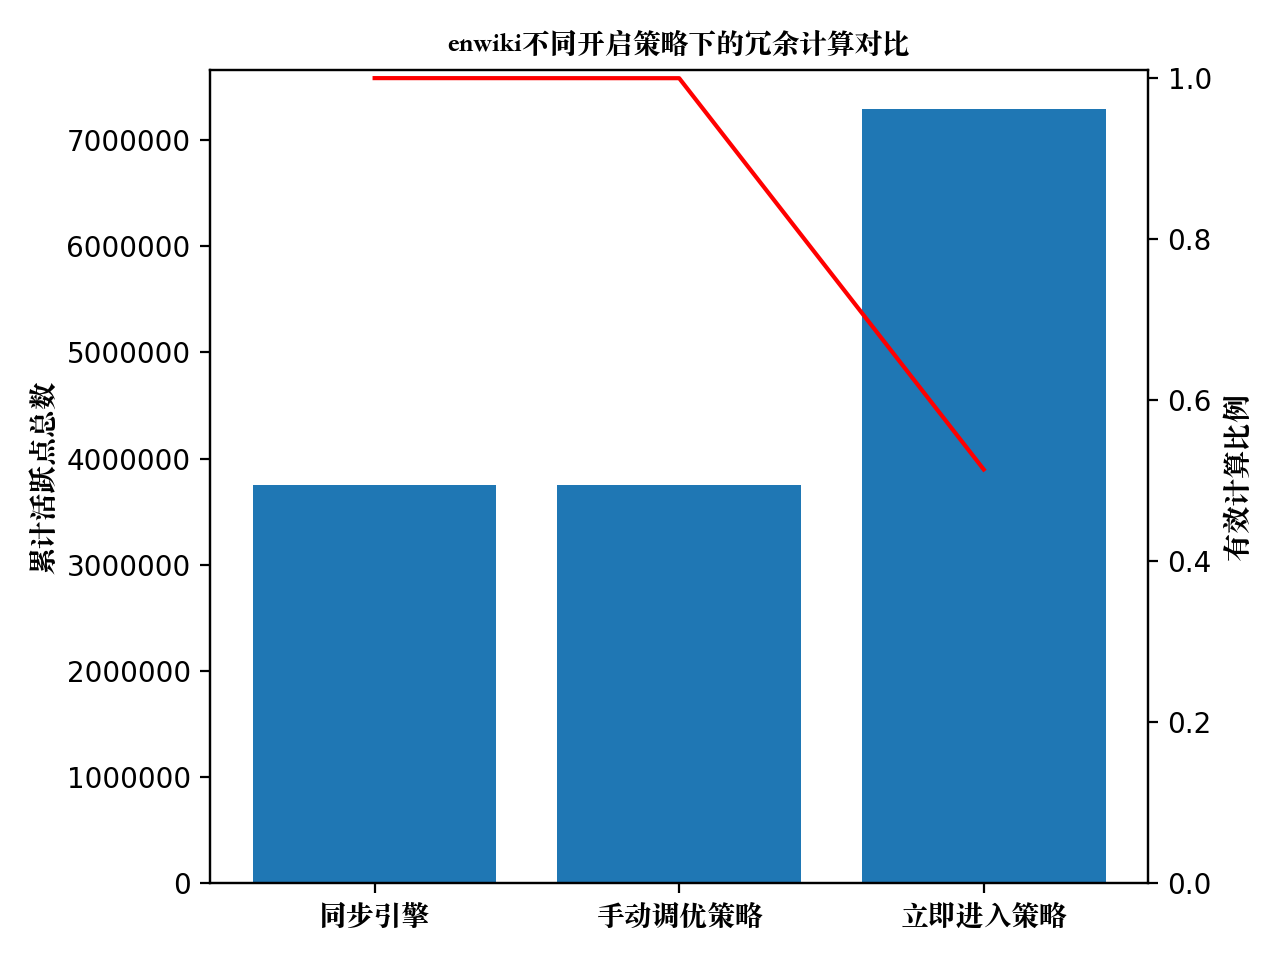
\includegraphics[width=\textwidth]{enwikiuseful}
    \caption{}
    % \label{fig:oaspl_a}
  \end{subfigure}%
  ~% add desired spacing
  \begin{subfigure}[b]{0.4\textwidth}
    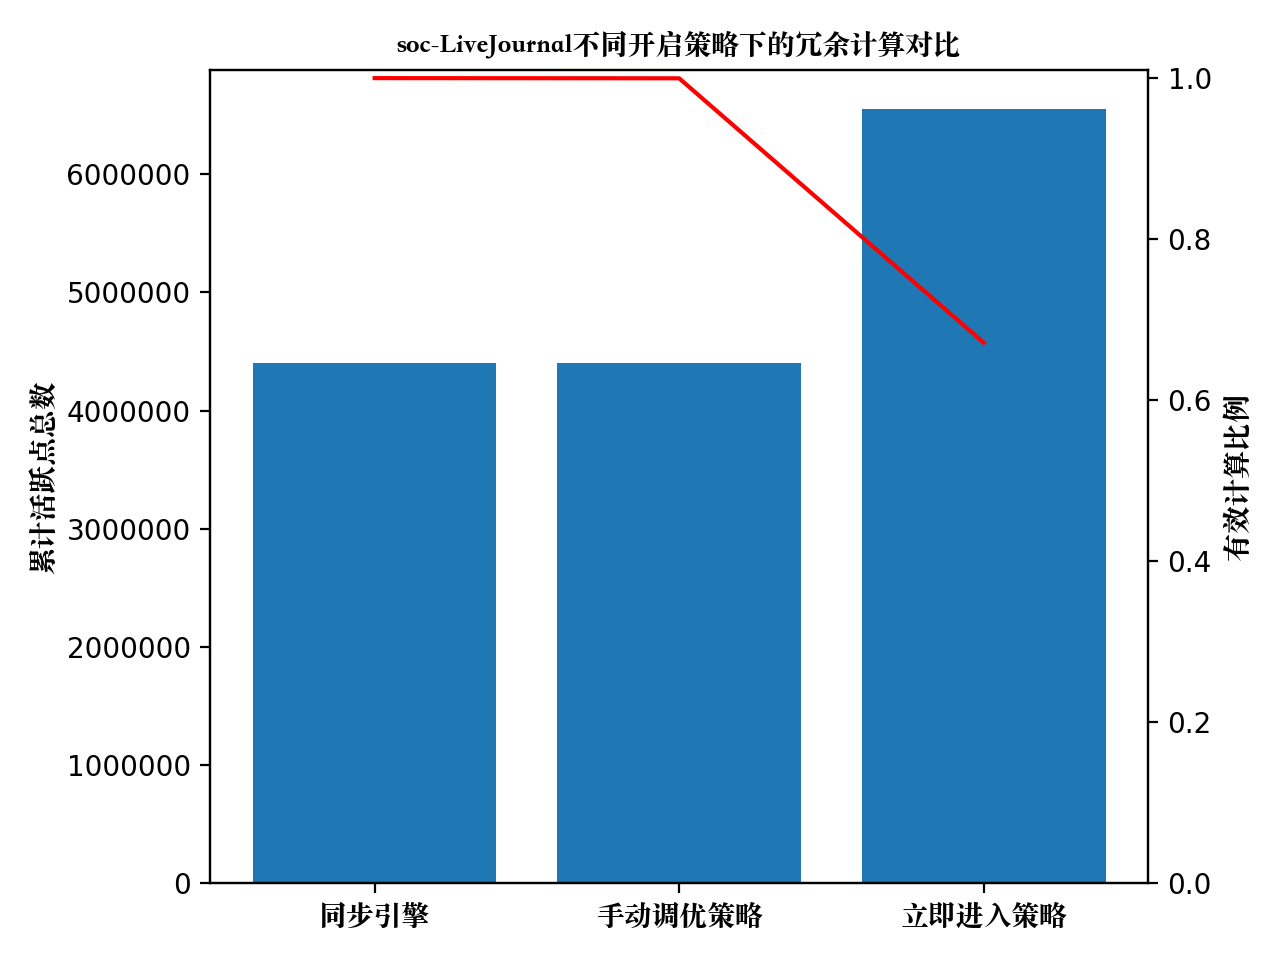
\includegraphics[width=\textwidth]{soc-LiveJournaluseful}
    \caption{}
    % \label{fig:oaspl_b}
  \end{subfigure}
  \\% line break
  \begin{subfigure}[b]{0.4\textwidth}
    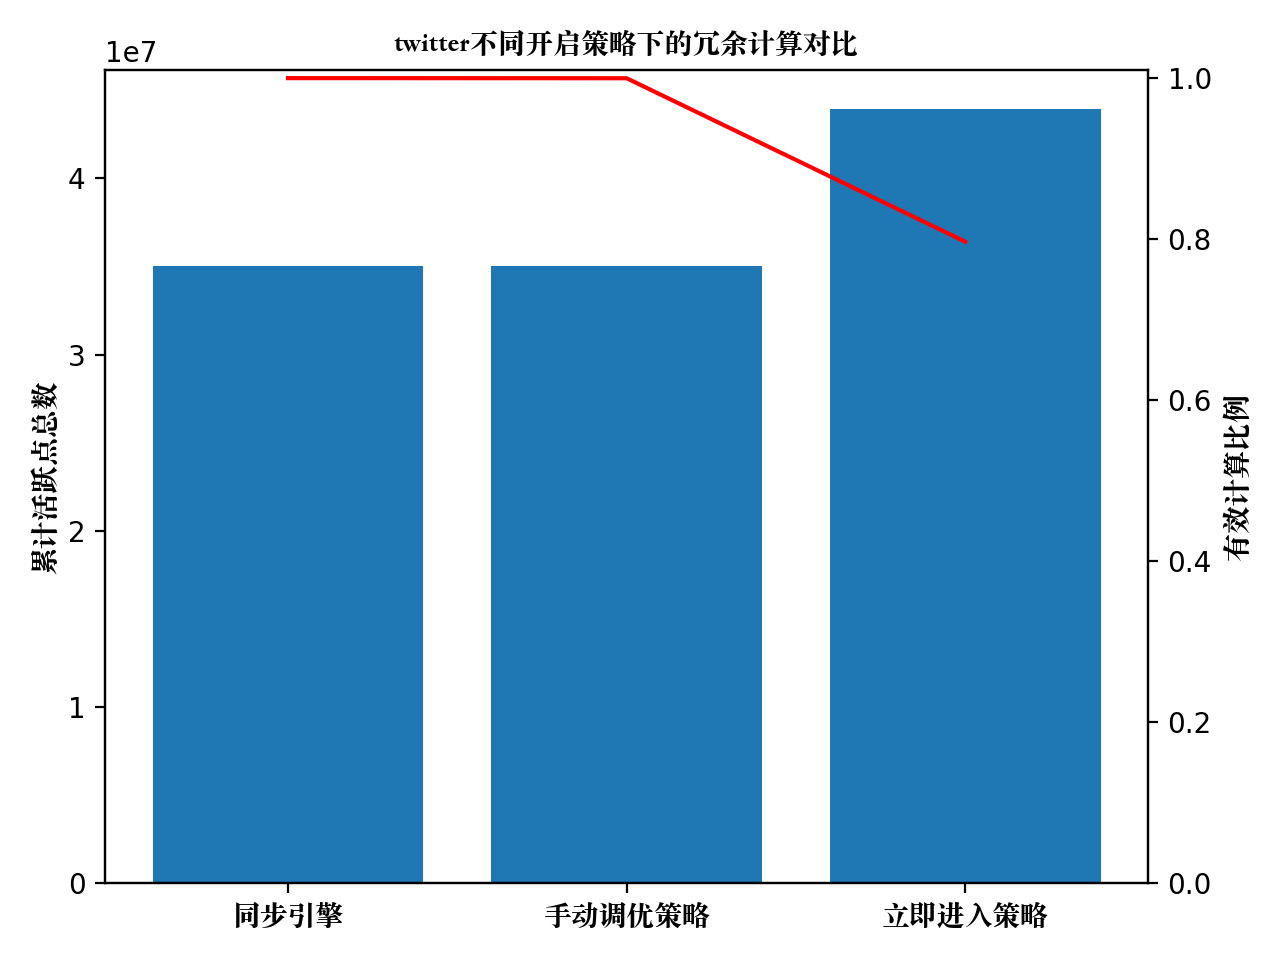
\includegraphics[width=\textwidth]{twitteruseful}
    \caption{}
    % \label{fig:oaspl_c}
  \end{subfigure}%
  ~% add desired spacing
  \begin{subfigure}[b]{0.4\textwidth}
    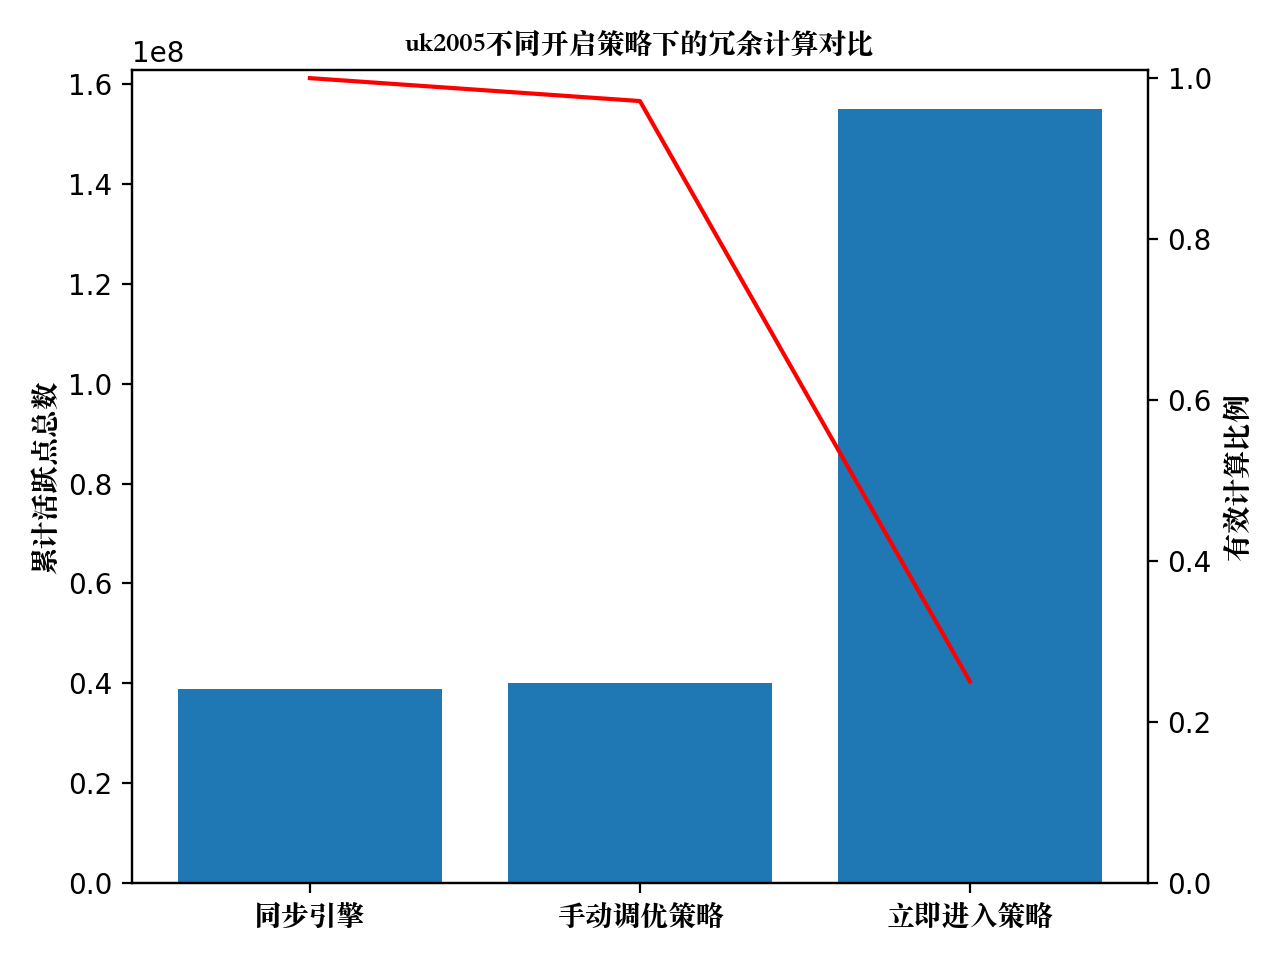
\includegraphics[width=\textwidth]{uk2005useful}
    \caption{}
    % \label{fig:oaspl_d}
  \end{subfigure}
  \bicaption{SSSP 算法在四个图上的冗余计算的比例}{The ratio of redundant calculation of SSSP algorithm on four graphs}
  \label{fig:useful}
\end{figure}
图\ref{fig:useful}给出了SSSP算法在4个本地性不好的图上的实验结果。
图中给出了采用eager data coherence 方法的同步引擎,手动调优策略的延迟数据一致性方法,立即进入策略的延迟数据一致性方法
这三种情况下,系统在整个计算过程中累计激活的活跃点的数据,和其中有效计算的比例。
同步引擎下由于采用了eager data coherence 方法所以其有效计算的比例总为1,其激活的活跃点的数目也代表了实际需要计算的活跃点的数目,
所以同步引擎的数据是基准数据。
以 SSSP 算法在 enwiki 这个图上的结果为例,我们可以看到在立即进入的策略下,延迟数据一致性方法所进行的有效计算的比例约为50\%,
也就是说这种策略下冗余计算的比例为50\%,有一半数量的活跃点上所进行的计算是无效的。
在具体的实验中甚至可看到,在第2轮中,系统激活并计算了156万个活跃点,但是只有6万个活跃点上的计算是正确有效的,
剩下的150万个点上的计算都是无效的,其有效计算的比例只有4\%,
像这样的本地计算带来的显然绝大部分都是性能损耗而不是收益。
而在手动调优之后,延迟数据一致性方法所进行的有效计算的比例为99.991\%,系统只对327个顶点进行了冗余计算。
可以看到手动调优之所以得到了更好的性能提升就是因为极大的减少了系统中存在的冗余计算的比例。


\begin{table}[!htbp]
  \bicaption{调优效果}{tuning effect}
  \label{tab:tuning}
  \centering
  \footnotesize% fontsize
  \setlength{\tabcolsep}{4pt}% column separation
  \renewcommand{\arraystretch}{1.2}%row space 
  \begin{subtable}[t]{0.45\textwidth}
      \centering
      \bicaption{enwiki 上的调优效果}{tuning effect on enwiki }
      \label{tab:sample_1}
      \begin{tabular}{lccc}
          \hline
          & iter  & time(s) \\
          \hline
          sync & 53 & 14.24 \\
          \hline
          lazyasync ,before tuning & 39 & 12.22 \\
          \hline
          lazyasync ,after tuning & 40 & 9.39 \\
          \hline
      \end{tabular}
  \end{subtable}
  ~% add desired spacing
  \begin{subtable}[t]{0.45\textwidth}
      \centering
      \bicaption{soc-Livejournal 上的调优效果}{tuning effect on soc-Livejournal }
      \label{tab:sample_2}
      \begin{tabular}{lccc}
          \hline
          & iter & time(s) \\
          \hline
          sync & 15 & 5.84 \\
          \hline
          lazyasync ,before tuning & 10 & 5.07 \\
          \hline
          lazyasync ,after tuning & 13 & 4.21 \\
          \hline
      \end{tabular}
  \end{subtable}
  \\% line break
  \begin{subtable}[t]{0.45\textwidth}
      \centering
      \bicaption{twitter 上的调优效果}{tuning effect on twitter }
      \label{tab:sample_3}
      \begin{tabular}{lccc}
          \hline
          & iter  & time(s) \\
          \hline
          sync & 13& 31.63 \\
          \hline
          lazyasync ,before tuning & 12 & 35.98 \\
          \hline
          lazyasync ,after tuning & 12 & 24.09 \\
          \hline
      \end{tabular}
  \end{subtable}
  ~% add desired spacing
  \begin{subtable}[t]{0.45\textwidth}
      \centering
      \bicaption{uk-2005 上的调优效果}{tuning effect on uk-2005 }
      \label{tab:sample_4}
      \begin{tabular}{lccc}
          \hline
          & iter  & time(s) \\
          \hline
          sync & 201 & 53.07 \\
          \hline
          lazyasync ,before tuning & 58 & 56.14 \\
          \hline
          lazyasync ,after tuning & 71 & 24.99 \\
          \hline
      \end{tabular}
  \end{subtable}
\end{table}
表\ref{tab:tuning}则给出了对应的SSSP算法在这4个图上手动调优前后的迭代次数和计算时间。
可以看到在四个大图上,相较于同步引擎,无论是立即进入策略还是手动调优,延迟数据一致性方法都减少了迭代次数和计算时间,
不过在uk-2005这个图上,立即进入策略相比同步引擎虽然减少了迭代次数,但是总的计算时间却增加了一点。
对比立即进入策略和手动调优策略, 可以看到手动调优之后虽然迭代次数相较于立即进入反而多了,但是最终的计算时间却进一步变少了。
这再次印证之前所提到的公式$T=iter \times t_{per\_iter}$,即计算时间受迭代次数和单次迭代时间共同影响。
减少迭代次数和降低单次迭代时间都能提高图计算的执行效率,而手动调优正是找到了冗余计算相对较少的情况,降低了单次迭代的时间。

% \begin{center}
%   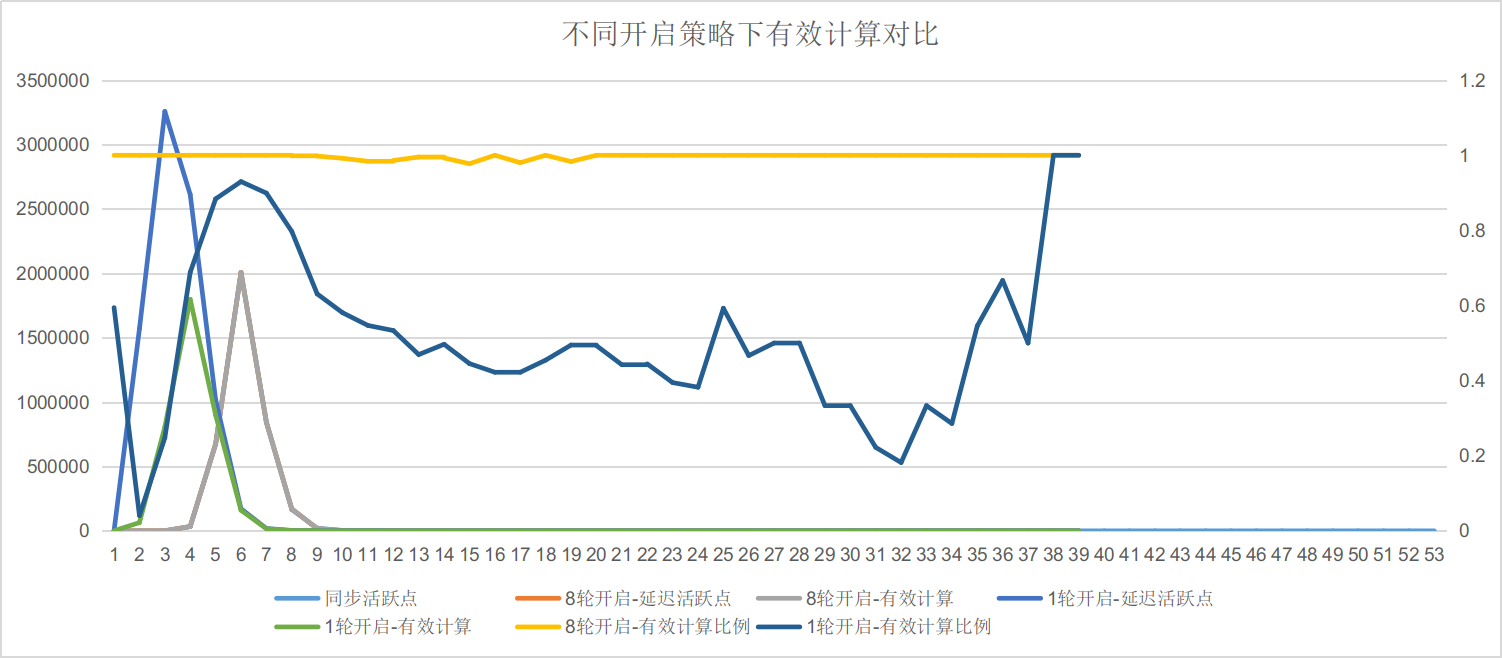
\includegraphics[width=0.8\textwidth]{wiki-lazy.png}
%   \captionof{figure}{enwiki图上不同的开启策略下的有效计算的比例}
%   \label{fig:wiki-lazy}
% \end{center}  

%2020.03.25 02:00

\section{本章小结}
在本章中,通过在小图上的具体分析和大图上的实验,我们发现延迟数据一致性方法所得到的性能提升程度和冗余计算的比例有关。
延迟数据一致性方法避免了原有的 eager data coherence 方法中存在的冗余同步,等待和通信,但是在自己的本地计算中引入了新的冗余计算。
这种冗余计算主要来自于延迟落后的数据在本地所进行的不必要的多轮计算,使得单次迭代的时间增加,最终影响了延迟数据一致性方法的性能提升。
在之前的工作中,我们先是手动调优找到延迟数据一致性方法相对最好的性能提升,然后用数据拟合的方法得到一个决策树策略。
但是这些都不能直接指导我们如何得到相对最优的性能提升,
现在我们发现延迟数据一致性方法可以通过降低冗余计算比例的方法来得到相对更好的性能提升。
